%%%%%%%%%%%%%%%%%%%%%%%%%%%%%%%%%%%%%%%%%%%%%%%%%%%%%%%%%%%%%%%

% Set up document

\documentclass{beamer}
\usecolortheme{whale}
\setbeamersize{text margin left=5mm,text margin right=5mm}

% Used to create a section slide between section
\AtBeginSection[]{
  \begin{frame}
  \vfill
  \centering
  \begin{beamercolorbox}[sep=8pt,center,shadow=true,rounded=true]{title}
    \usebeamerfont{title}\insertsectionhead\par%
  \end{beamercolorbox}
  \vfill
  \end{frame}
}

% Remove default navigation symbols and add just  page number
\setbeamertemplate{navigation symbols}{} % Clear default navigation
\addtobeamertemplate{navigation symbols}{}{%
    \usebeamerfont{footline}%
    \usebeamercolor[fg]{footline}%
    \hspace{1em}%
    \insertframenumber/\inserttotalframenumber
}

%%%%%%%%%%%%%%%%%%%%%%%%%%%%%%%%%%%%%%%%%%%%%%%%%%%%%%%%%%%%%%%

% Title page

\title{What would other emergency stroke teams do?}
\subtitle{Using explainable machine learning to understand variation in thrombolysis practice}


\author{Kerry Pearn\inst{1}, Michael Allen\inst{1,3}, Anna Laws\inst{1}, Richard Everson\inst{3}, Martin James\inst{1,2} }
\institute{\inst{1}University of Exeter Medical School \inst{2}Royal Devon University Healthcare NHS Foundation Trust \inst{3}University of Exeter Institute of Data Science and Artificial Intelligence}

%\institute{Overleaf}
%\date{March 2023}


\begin{document}

%\frame{\titlepage}

\begin{frame}
\titlepage

\end{frame}

%%%%%%%%%%%%%%%%%%%%%%%%%%%%%%%%%%%%%%%%%%%%%%%%%%%%%%%%%%%%%%%

\begin{frame}
\frametitle{Stroke types}

Most stokes (at least four out of five) are caused by a clot in a blood vessel in the brain. This is also called an \emph{ischaemic} stroke.

\vspace{3mm}



\begin{center}
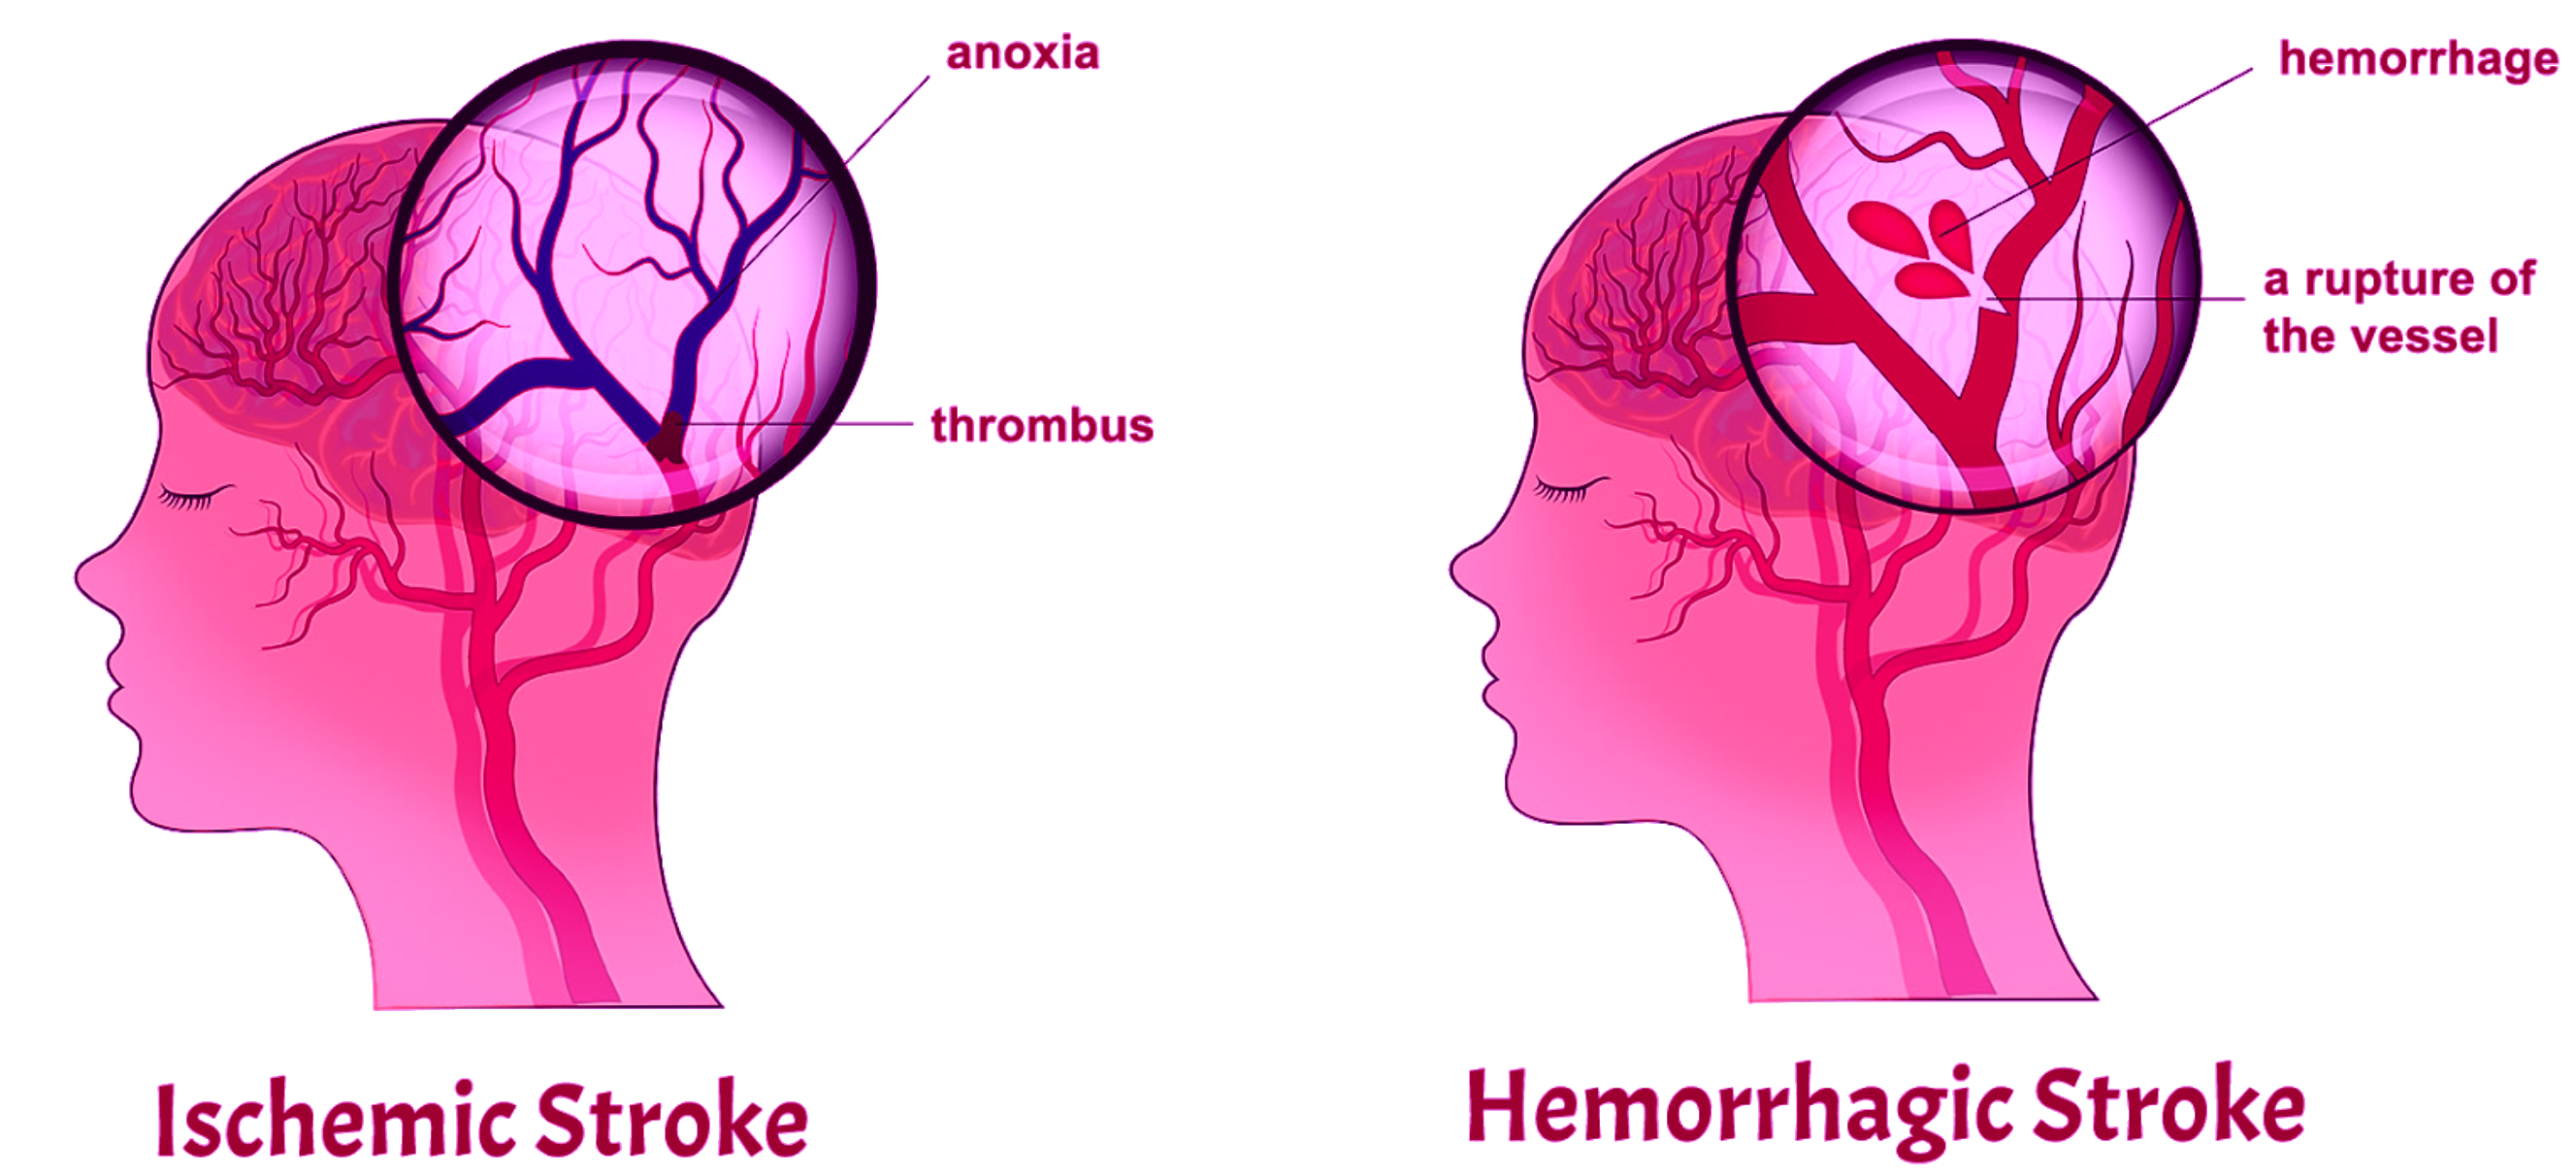
\includegraphics[width=1.0\textwidth]{./images/stroke_types}
\end{center}


\end{frame}
\begin{frame}
\frametitle{Thrombolysis (\emph{'Clot-busting'} medication) in stroke}

While the clot is still fresh, thrombolysis may be given to help break down the clot and restore blood flow.

\vspace{3mm}

\begin{center}
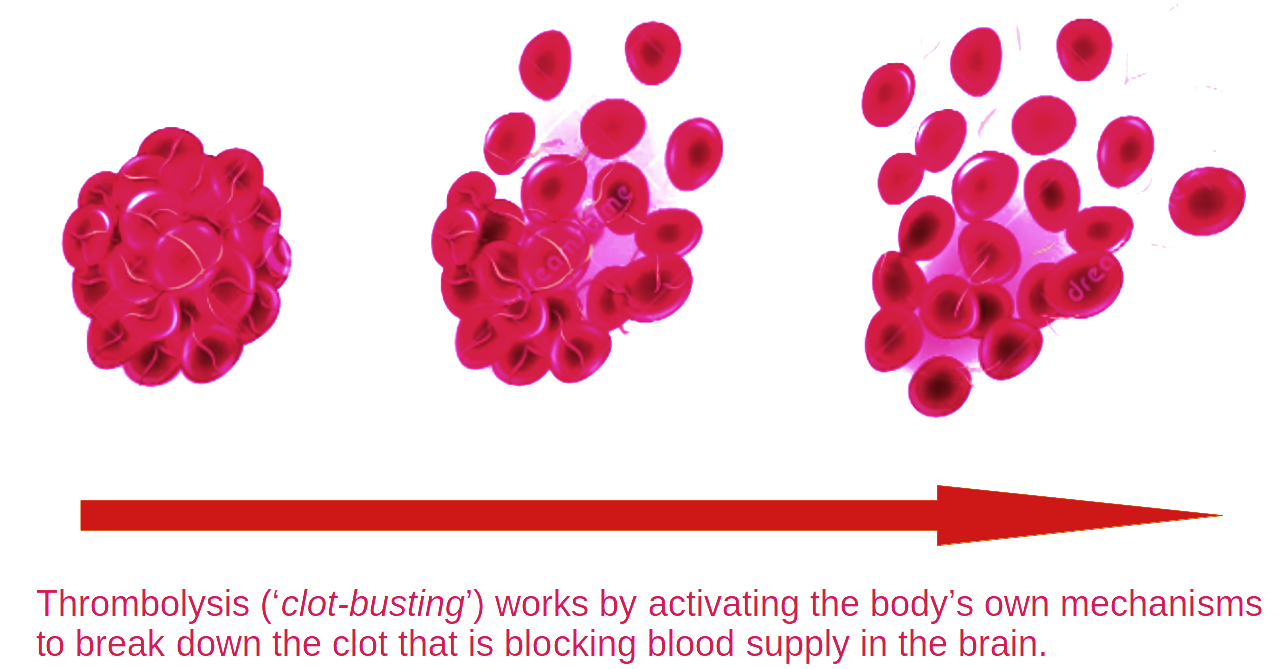
\includegraphics[width=0.70\textwidth]{./images/thrombolysis_mechanism}
\end{center}

\textbf{Drawbacks/limitations}: There is a risk of severe bleed (in about 1 in 50 patients on average, with risk increasing with stroke severity), and thrombolysis loses effectiveness over about the first 5-6 hours.

\end{frame}
\begin{frame}
\frametitle{Thrombolysis rates vary .... a lot}
Here is the range of thrombolysis use across the 132 acute stroke centres in England and Wales, 2016-2018.
\begin{center}
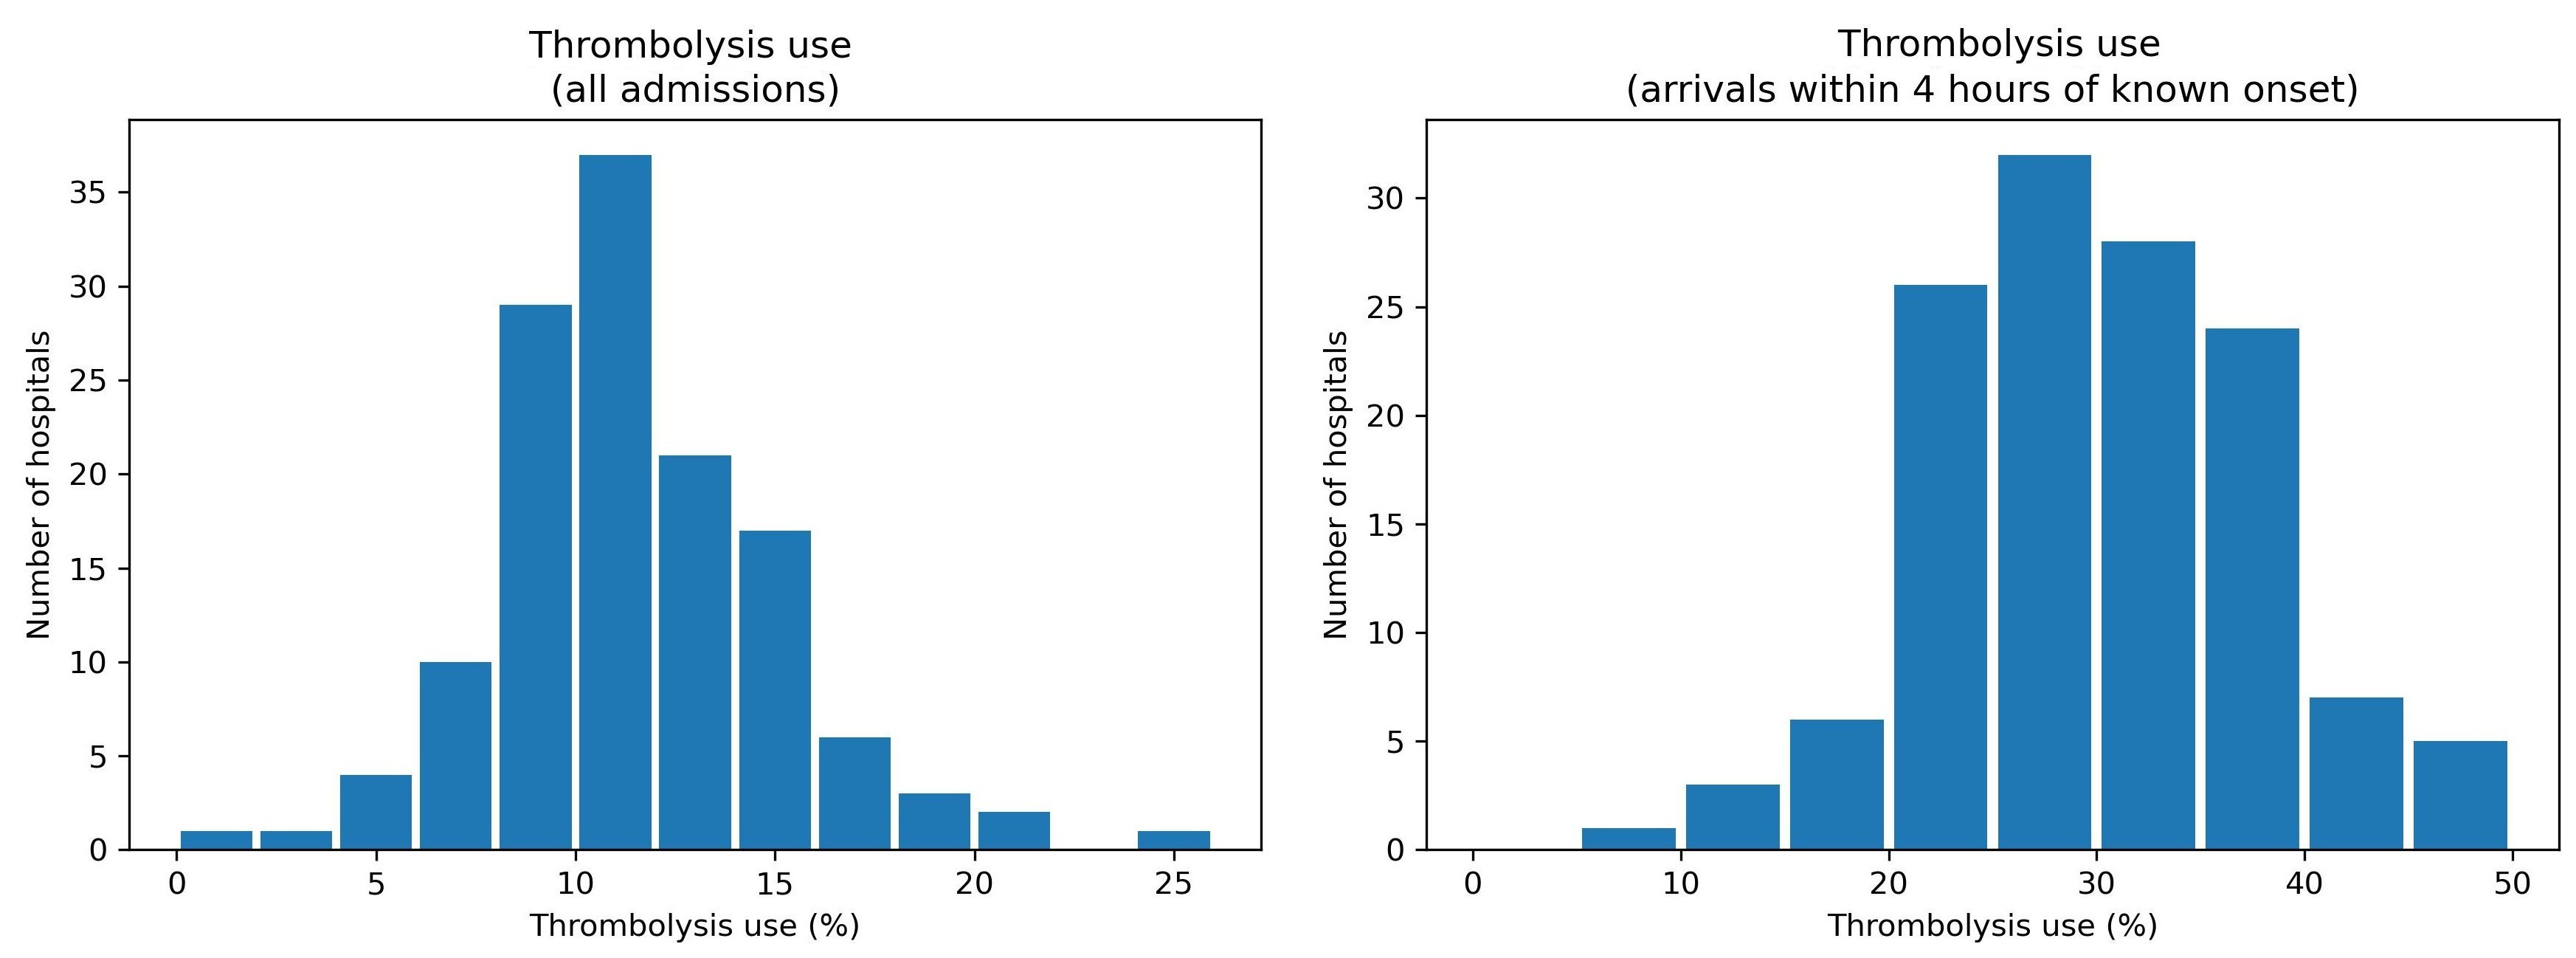
\includegraphics[width=1.0\textwidth]{./images/thrombolysis_hist}
\end{center}

How much of this variation is due to differences in local patient populations, and how much is due to differences in decisions hospitals make on who they would give thrombolysis to?
\end{frame}
\begin{frame}
\frametitle{Use of thrombolysis rates varies significantly between hospitals}

\small
Thrombolysis use varied from below 5\% to 25\% across the 132 acute stroke centres in England and Wales, 2016-2018.
\begin{center}
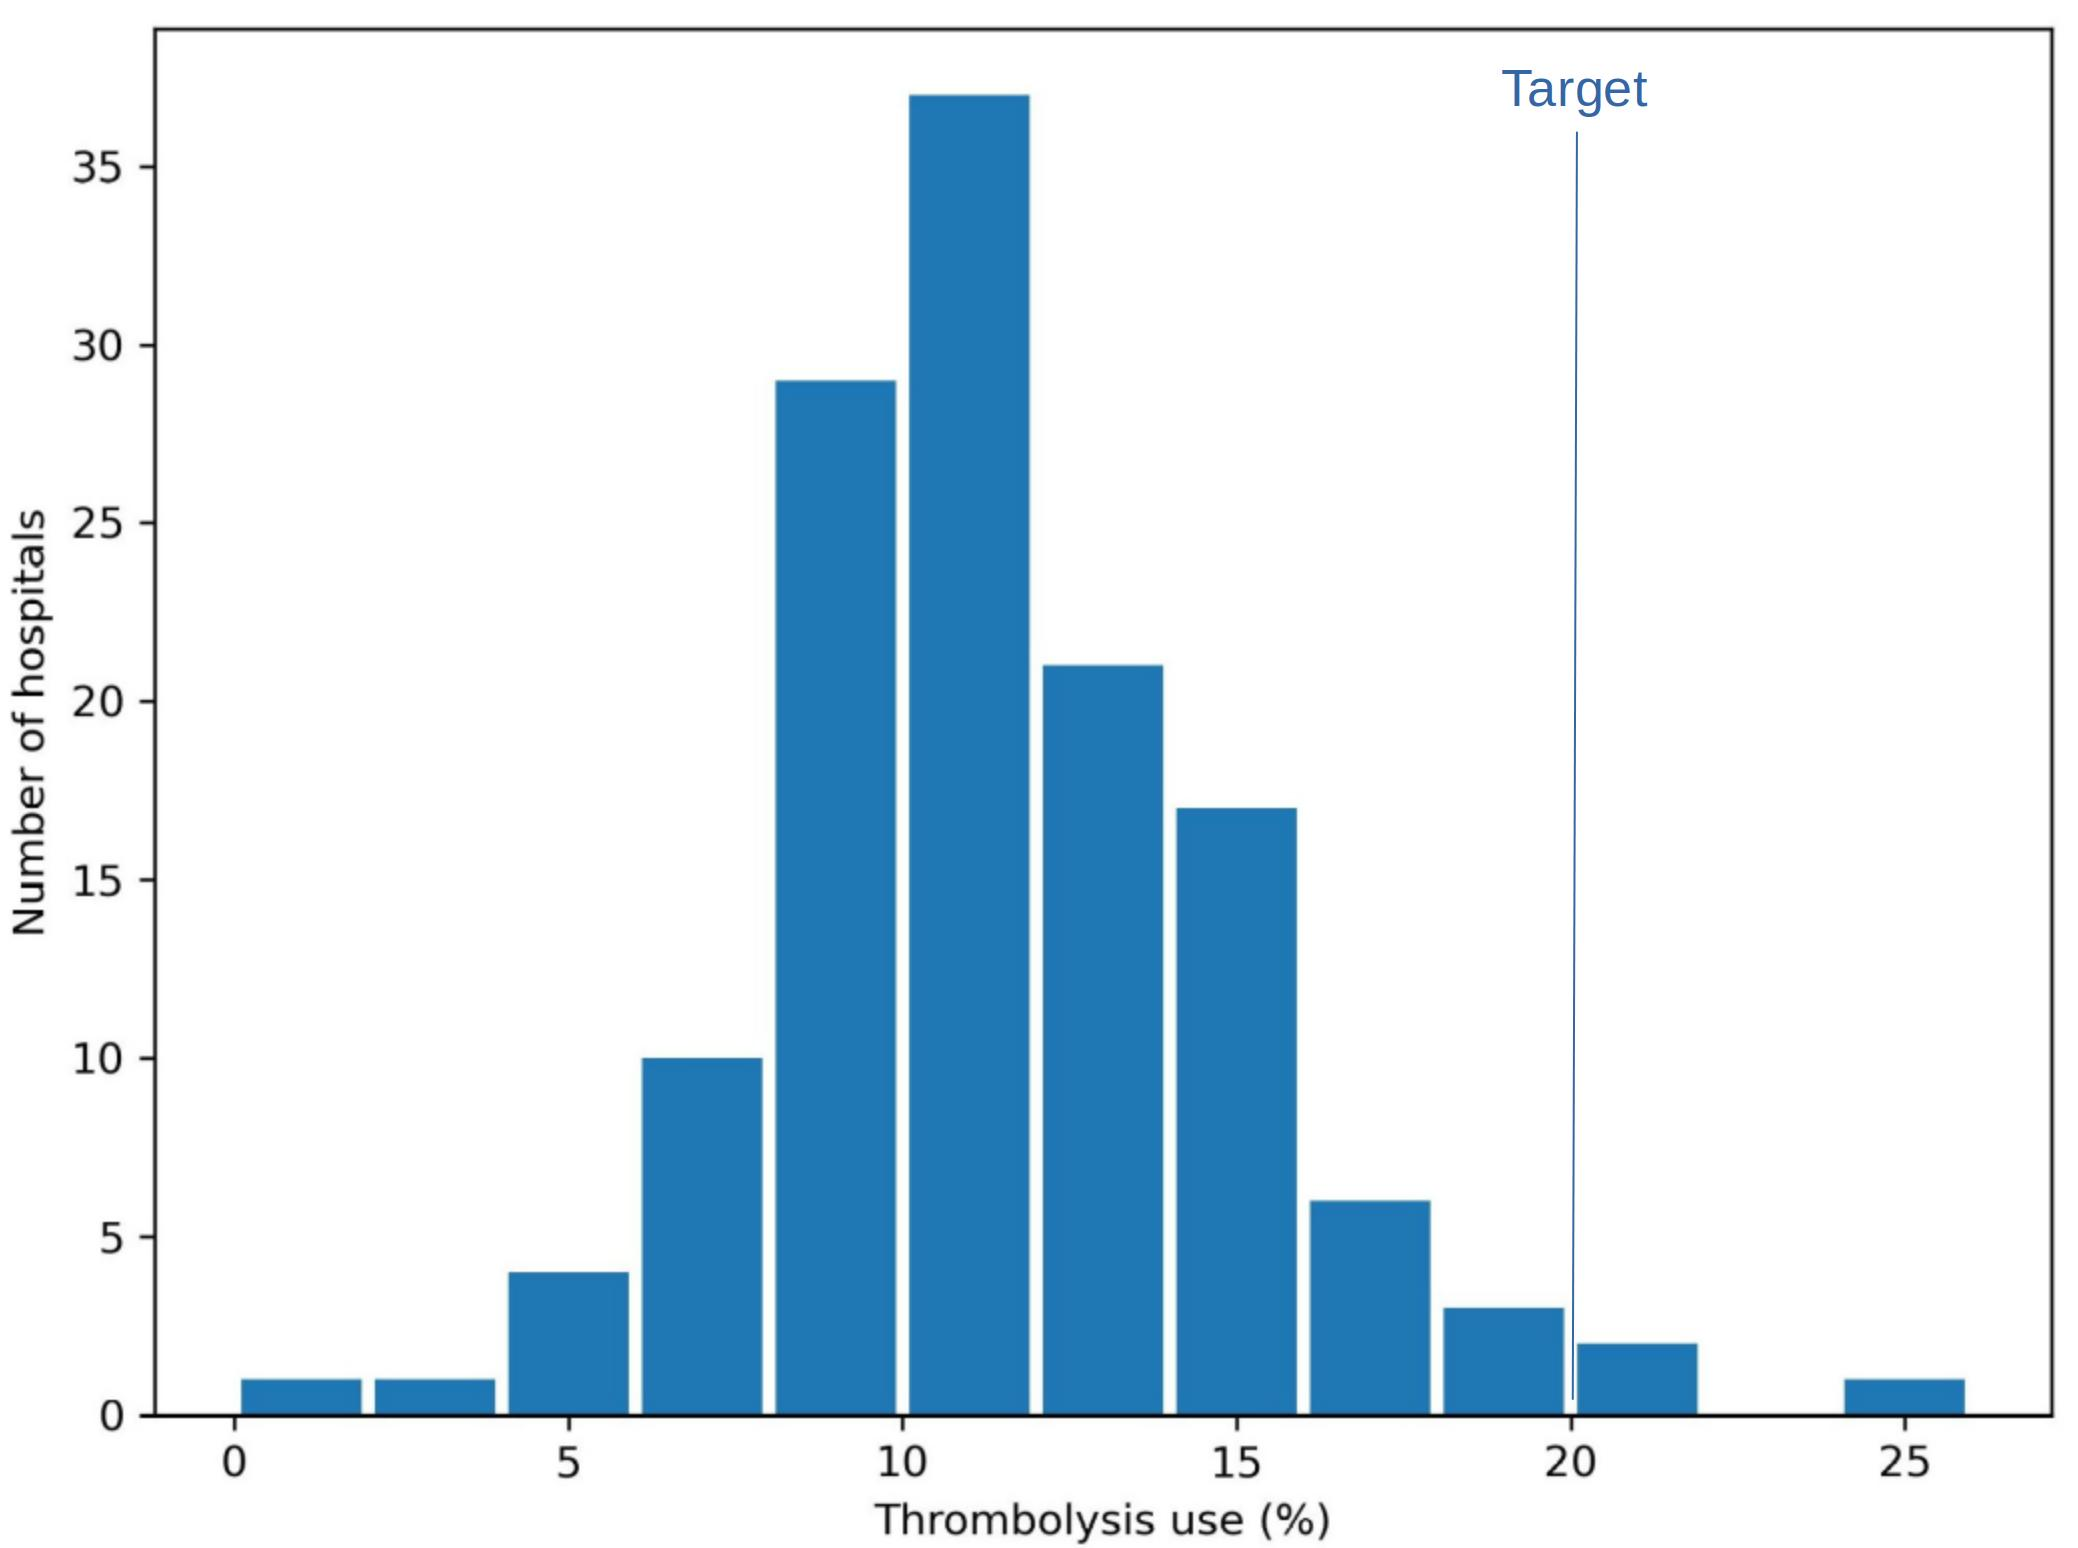
\includegraphics[width=0.50\textwidth]{./images/thrombolysis_by_hospital}
\end{center}

How much of this variation is due to differences in local patient populations, and how much is due to differences in in-hospital processes and decisions hospitals make on who they would give thrombolysis to?
\end{frame}
\begin{frame}
\frametitle{Breaking down the emergency stroke pathway into key steps}
\begin{center}
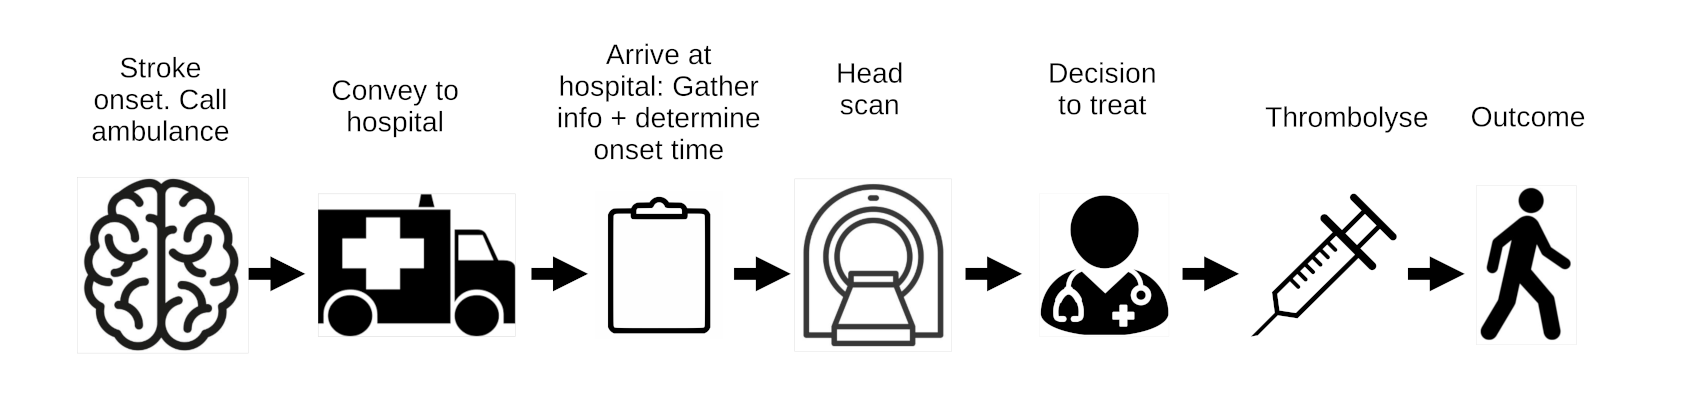
\includegraphics[width=1.0\textwidth]{./images/pathway}
\end{center}
We can model key changes to pathway, such as:
\begin{small}
\begin{itemize}
    \item What if the pathway were \textbf{faster}?
    \item What if hospital \textbf{determined the stroke onset time} in more patients?
    \item What if clinical \textbf{decision-making} was like that of \emph{benchmark} hospitals? (Predict what treatment a patient would receive at other hospitals).
\end{itemize}
\end{small}
\footnotesize{We model these changes with a hospital's own patient population, to allow for inter-hospital variation in patient population characteristics.}
\end{frame}
\begin{frame}
\frametitle{Our Approach}

\small

\begin{itemize}
    \item Train a machine learning algorithm to learn to predict to which patients each hospital would, or would not, give thrombolysis.
    \item Identify the patient characteristics which are most important in predicting use of thrombolysis, and produce a simpler machine learning model based on these characteristics.
    \item Identify \emph{ideal} candidates for thrombolysis.
    \item Add an \emph{explainable machine learning} layer* to understand patterns of use of thrombolysis.
    \item Investigate what we think would happen if every hospital received exactly the same 10k cohort of patients.
    \item Identify key subgroups of patients where hospitals differ in their use of thrombolysis.
\end{itemize}

\vspace{3mm}
\footnotesize
*SHAP (Shapley Additive Values, which provide information on what contribution each patient characteristic makes to the final prediction of whether they will, or will not, receive thrombolysis).
\end{frame}
\begin{frame}
\frametitle{Machine learning overview}
\begin{center}
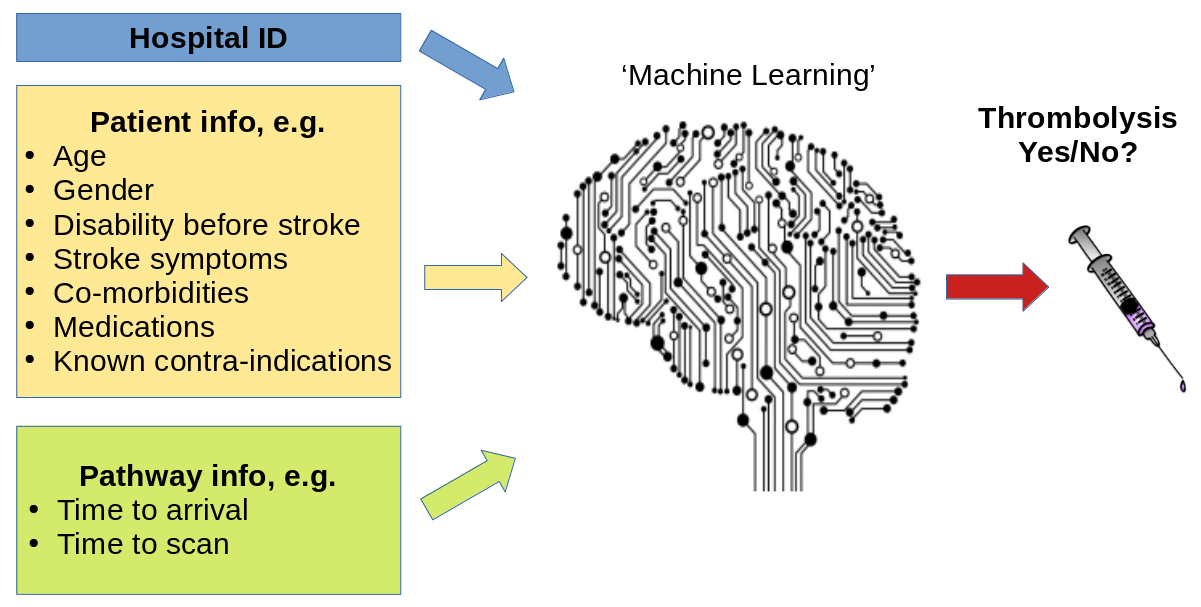
\includegraphics[width=0.80\textwidth]{./images/ml_model_high_level}
\end{center}

\small
\textbf{Machine learning is based on the simple principle of recognising similarity to what has been seen before.}
\vspace{2mm}

\footnotesize{We accessed 246,676 emergency stroke admissions in England and Wales over three years. Our machine learning models use XGBoost classification, and are based on those 88,928 patients who arrive within 4 hours of known stroke onset. Accuracy = 85\% (ROC AUC = 0.92).}
\end{frame}
\begin{frame}
\frametitle{Simplifying our model}

In order to simplify the model, to make it easier to explain, we reduced the number of patient features from 60 to 10, with almost no loss of model accuracy.

\small
\begin{itemize}
    \item \emph{Arrival-to-scan time}: Time from arrival at hospital to scan (mins)
    \item \emph{Infarction}: Stroke type (infarction or haemorrhage)
    \item \emph{Stroke severity}: Stroke severity (NIHSS) on arrival (ranges from 0 to 42)
    \item \emph{Precise onset time}: Onset time is known precisely
    \item \emph{Prior disability level}: Disability level (modified Rankin Scale) before stroke
    \item \emph{Stroke team}: Stroke team attended
    \item \emph{Use of AF anticoagulants}: Use of atrial fibrillation anticoagulant
    \item \emph{Onset-to-arrival time}: Time from onset of stroke to arrival at hospital
    \item \emph{Onset during sleep}: Did stroke occur in sleep?
    \item \emph{Age}: Age (as middle of 5 year age bands)
\end{itemize}
\end{frame}
\begin{frame}{Model accuracy, and simplification}

A model with all available 84 features had an ROC AUC of 0.922. A model with 10 features had an ROC AUC of 0.919.

\begin{center}
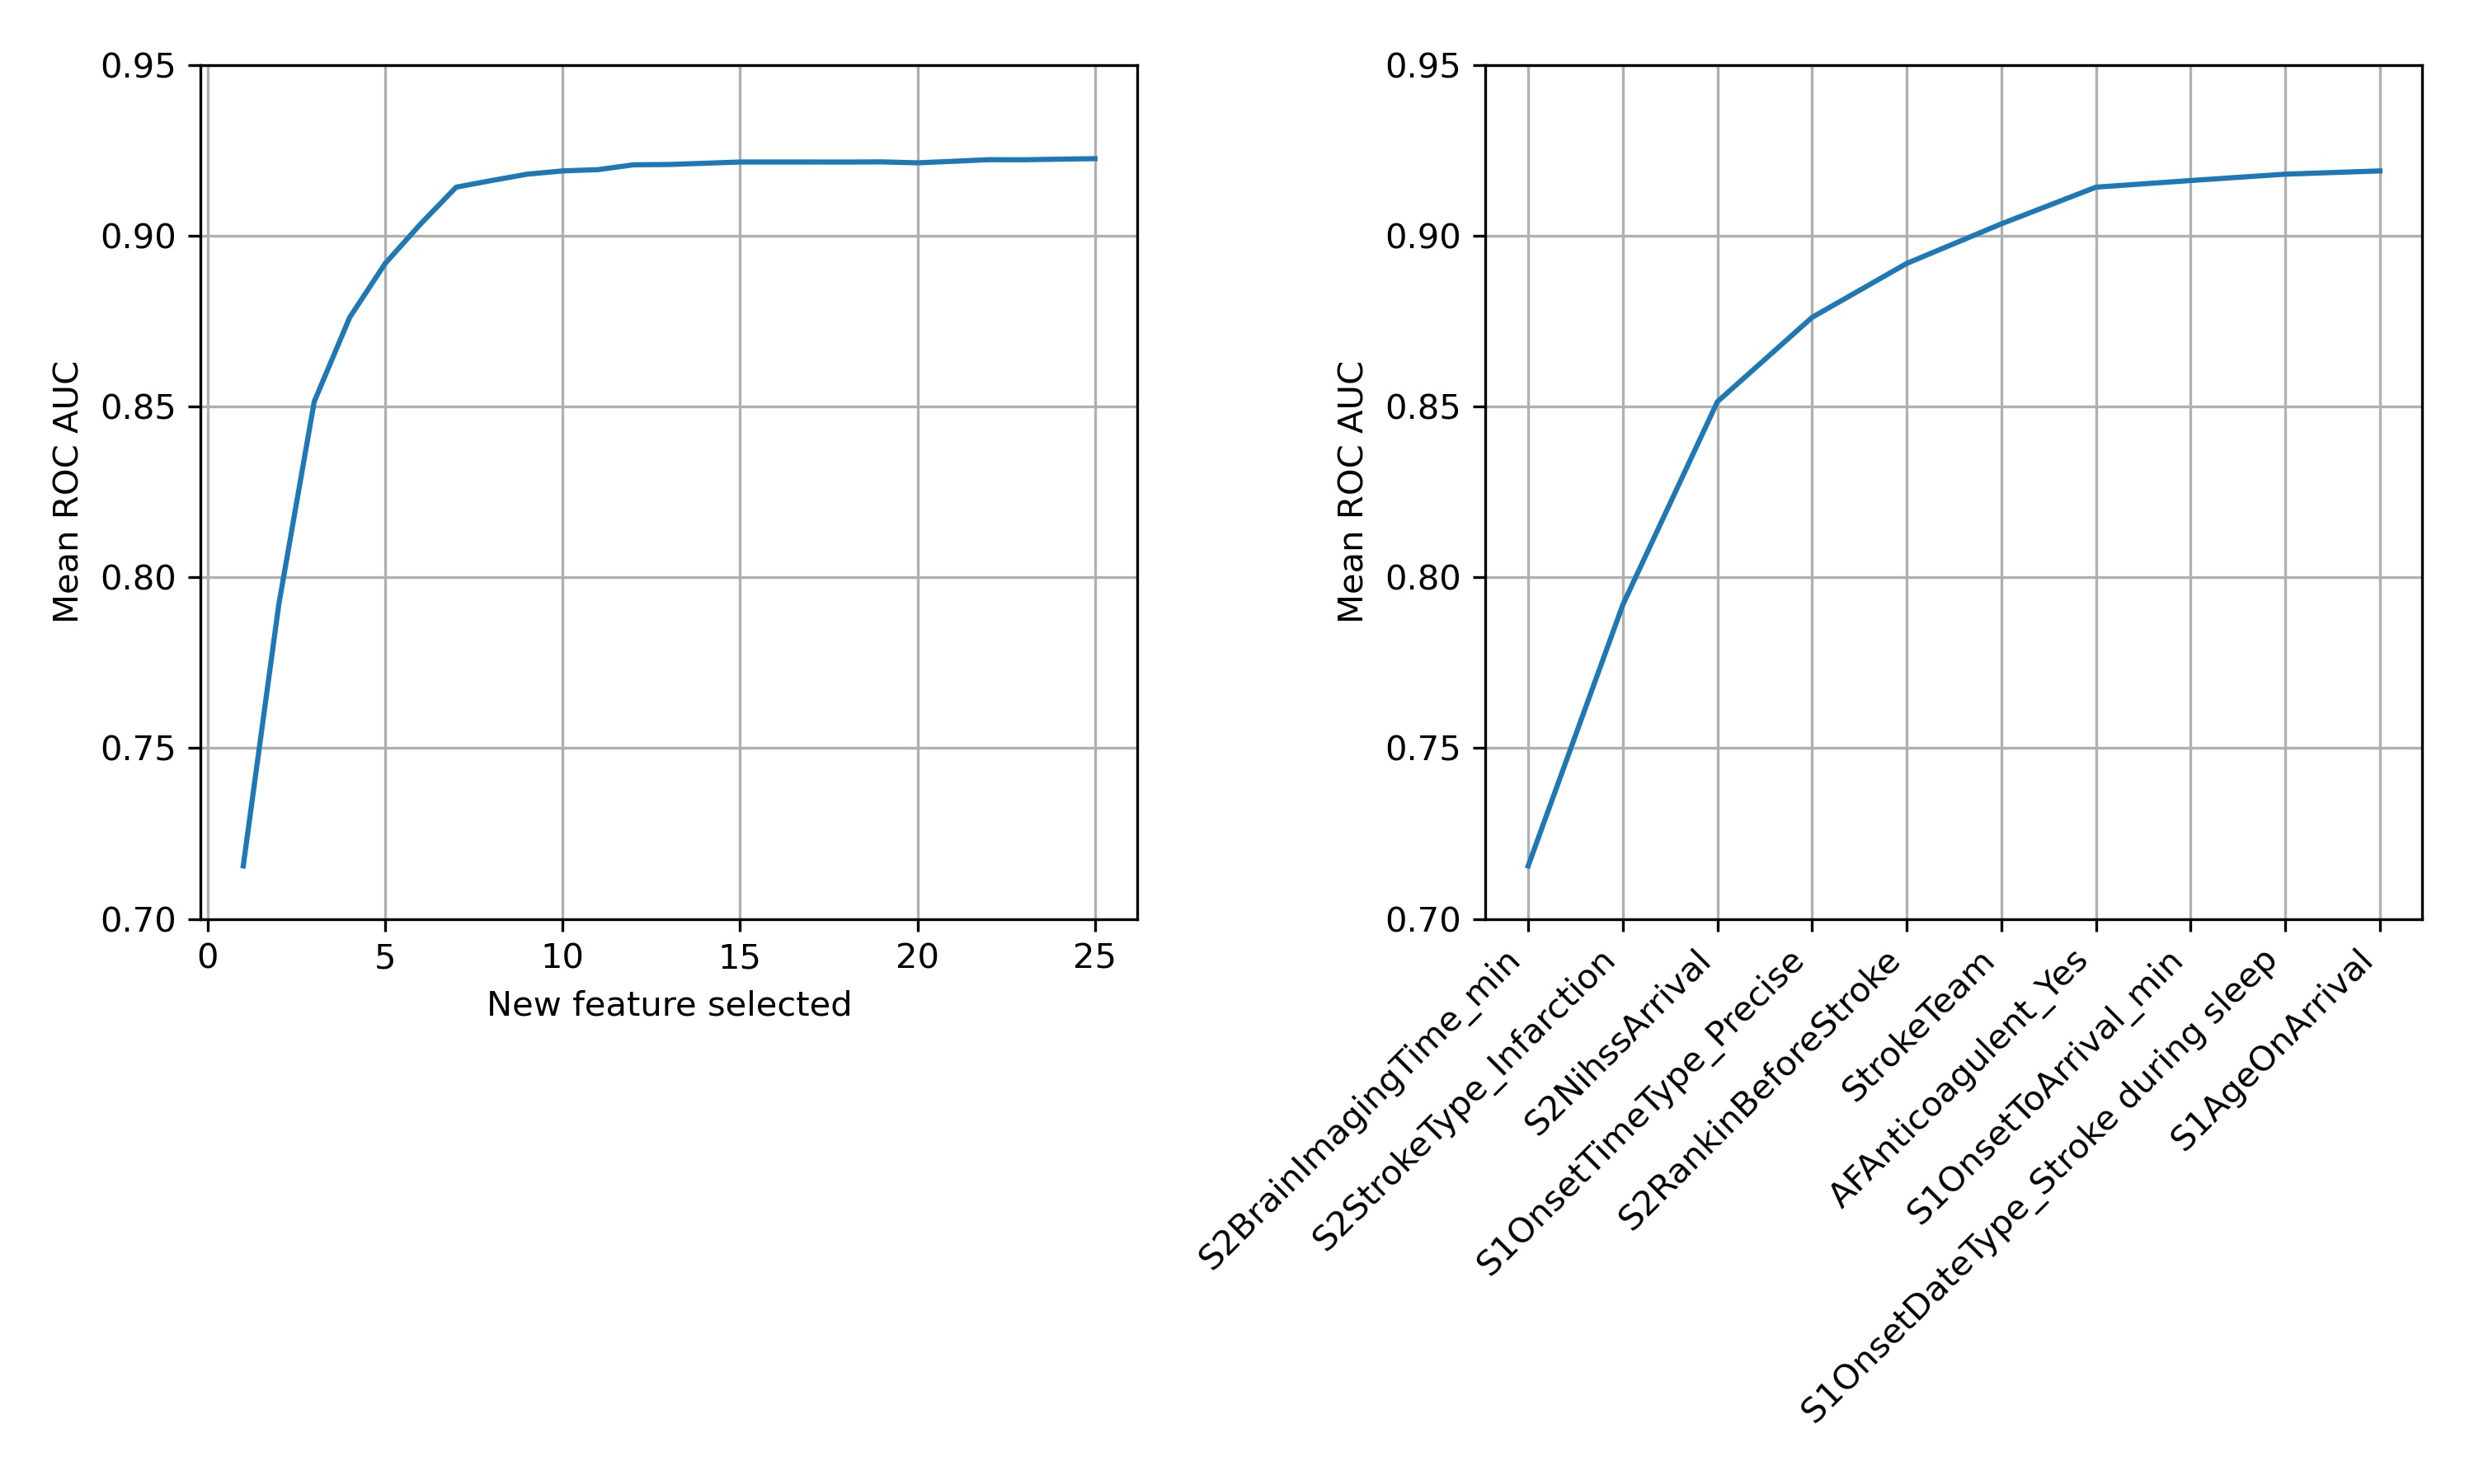
\includegraphics[width=0.9\textwidth]{./images/01_feature_selection.jpg}
\end{center}

Our simpler machine learning model will just use these 10 features.

\end{frame}
\begin{frame}{Predicting hospital thrombolysis use}

Predicted thrombolysis use was measured by combining 5 test sets from k-fold validation. The predicted vs. observed thrombolysis are highly correlated (r-squared 0.977). 

\begin{center}
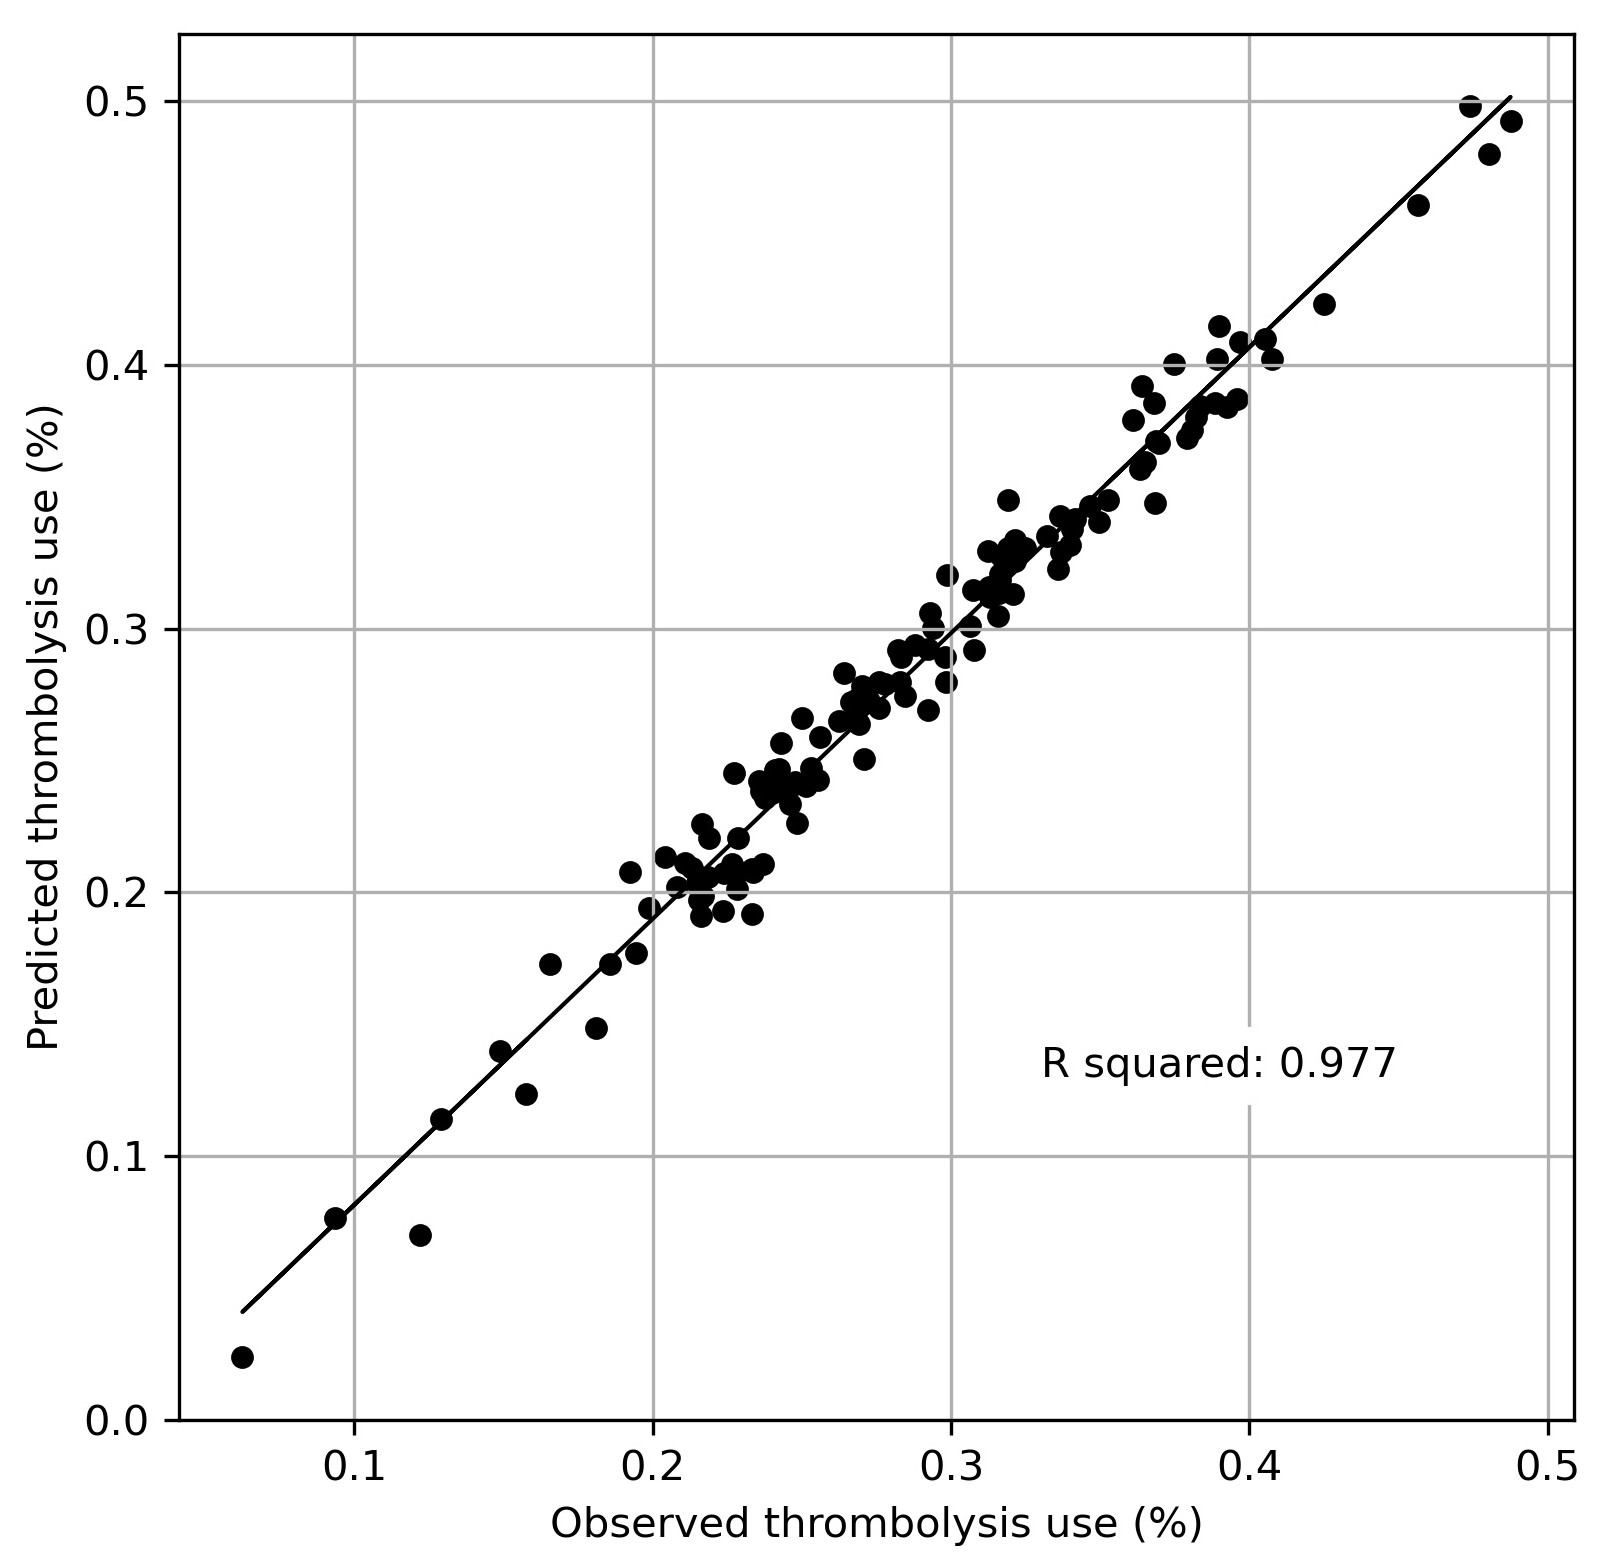
\includegraphics[width=0.55\textwidth]{./images/02_xgb_10_features_observed_predicted_rates.jpg}
\end{center}



\end{frame}
\begin{frame}{Model accuracy: Receiver Operating Characteristic Curve}


\begin{center}
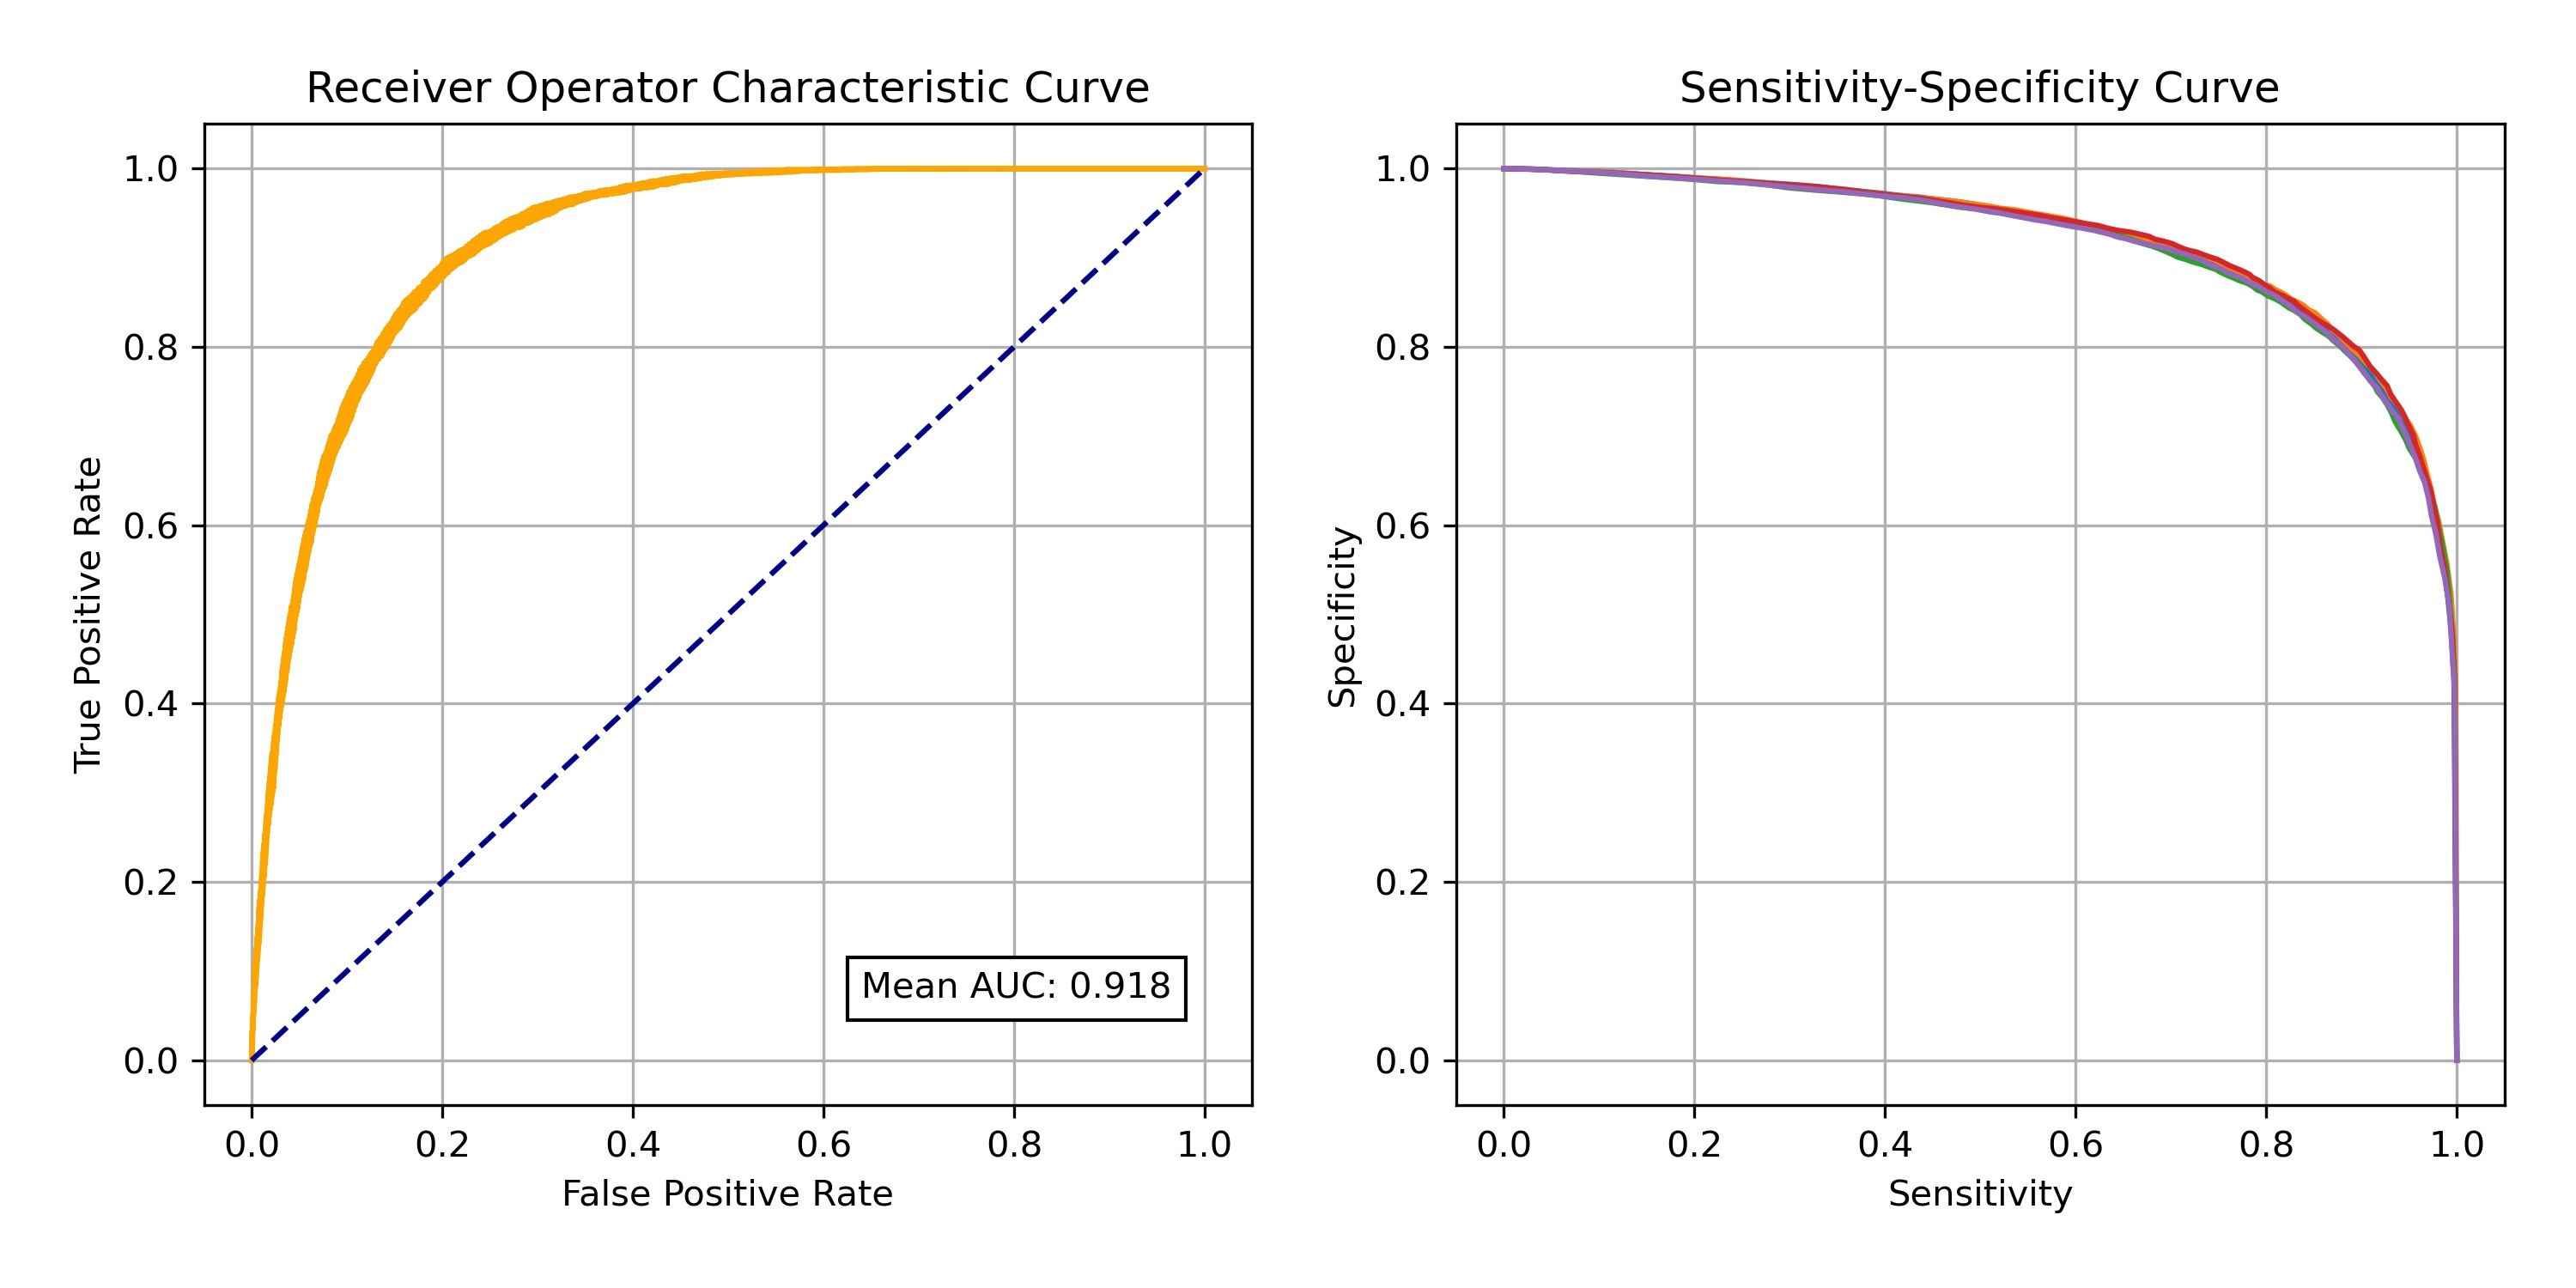
\includegraphics[width=0.9\textwidth]{02_xgb_10_features_roc_sens_spec}
\end{center}


\end{frame}
\begin{frame}{Model calibration}


\begin{center}
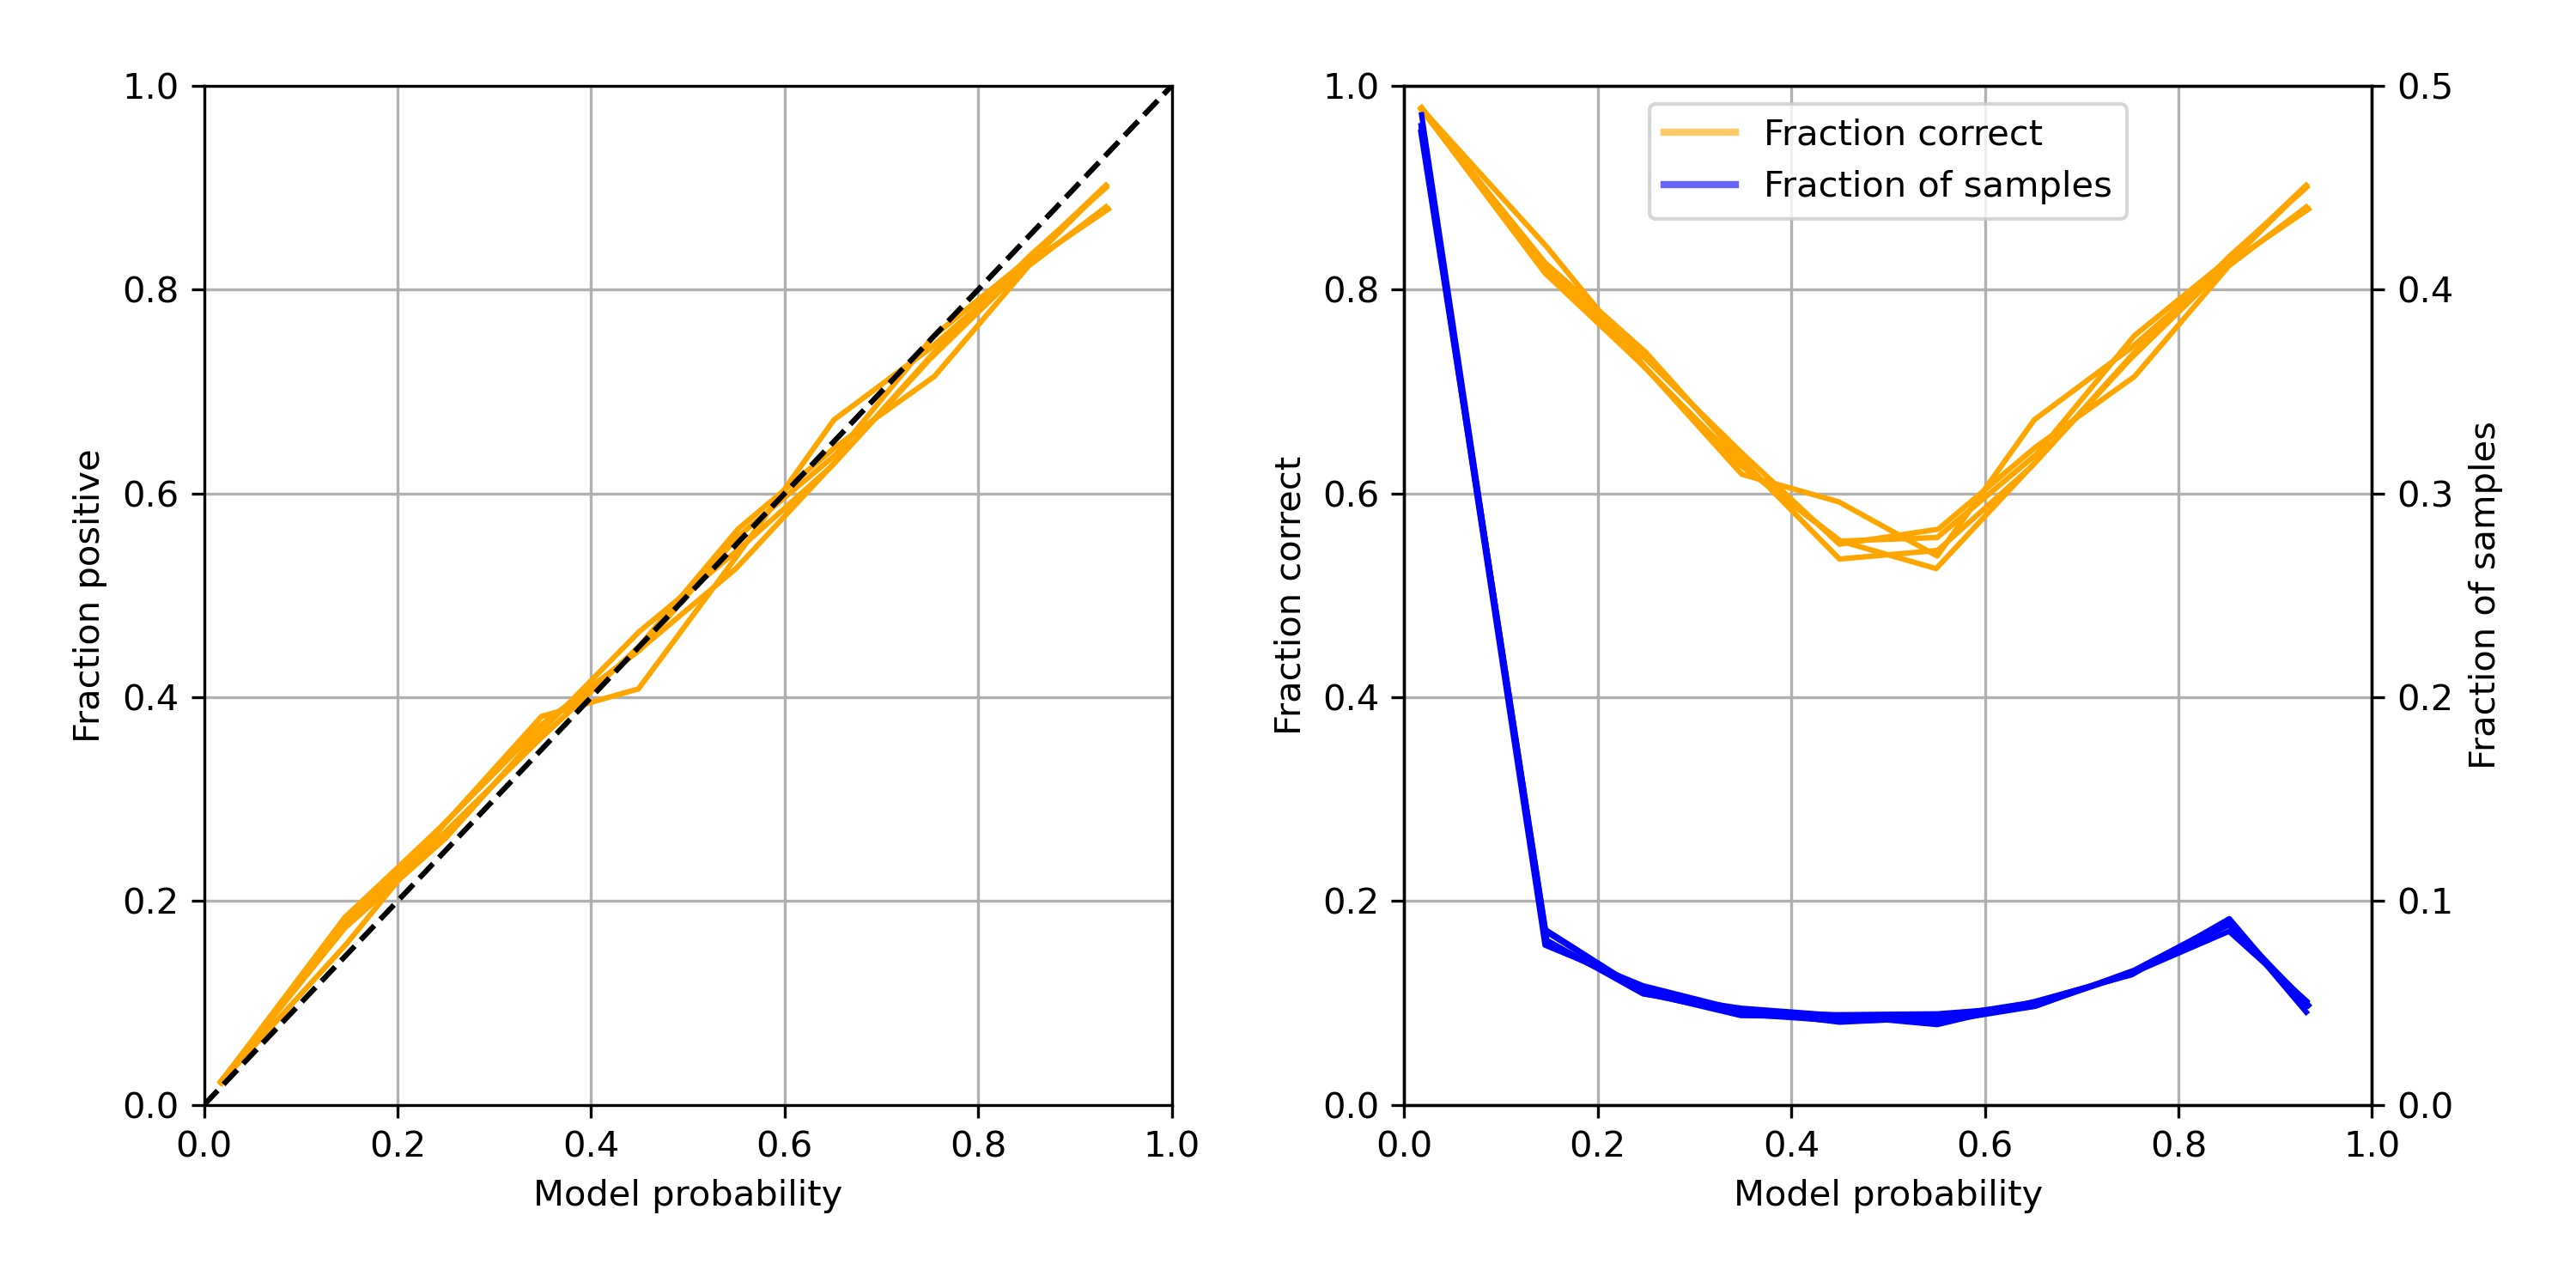
\includegraphics[width=1.0\textwidth]{./images/02_xgb_10_features_reliability}
\end{center}


\end{frame}
\begin{frame}
\frametitle{Explaining model predictions with SHAP values}

SHAP values show the influence of features (even for \emph{`black box'} models).

\begin{center}
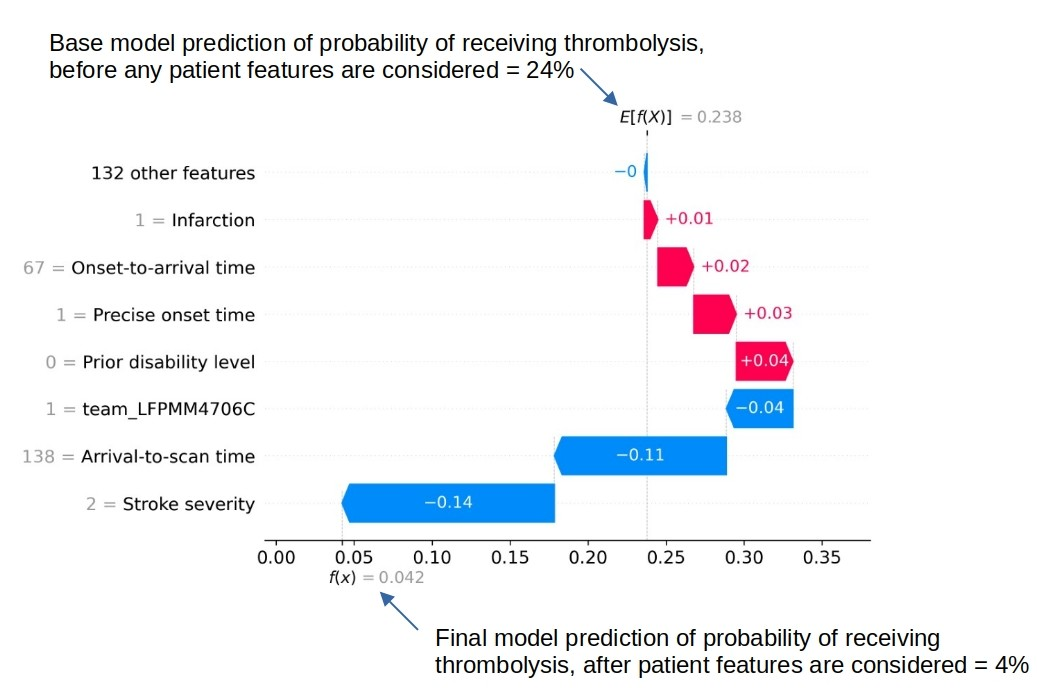
\includegraphics[width=0.90\textwidth]{./images/xgb_waterfall_low_probability_2.jpg}
\end{center}
\end{frame}
\begin{frame}
\frametitle{SHAP values for thrombolysis prediction}
Note: SHAP values here are log odds. 
\begin{center}
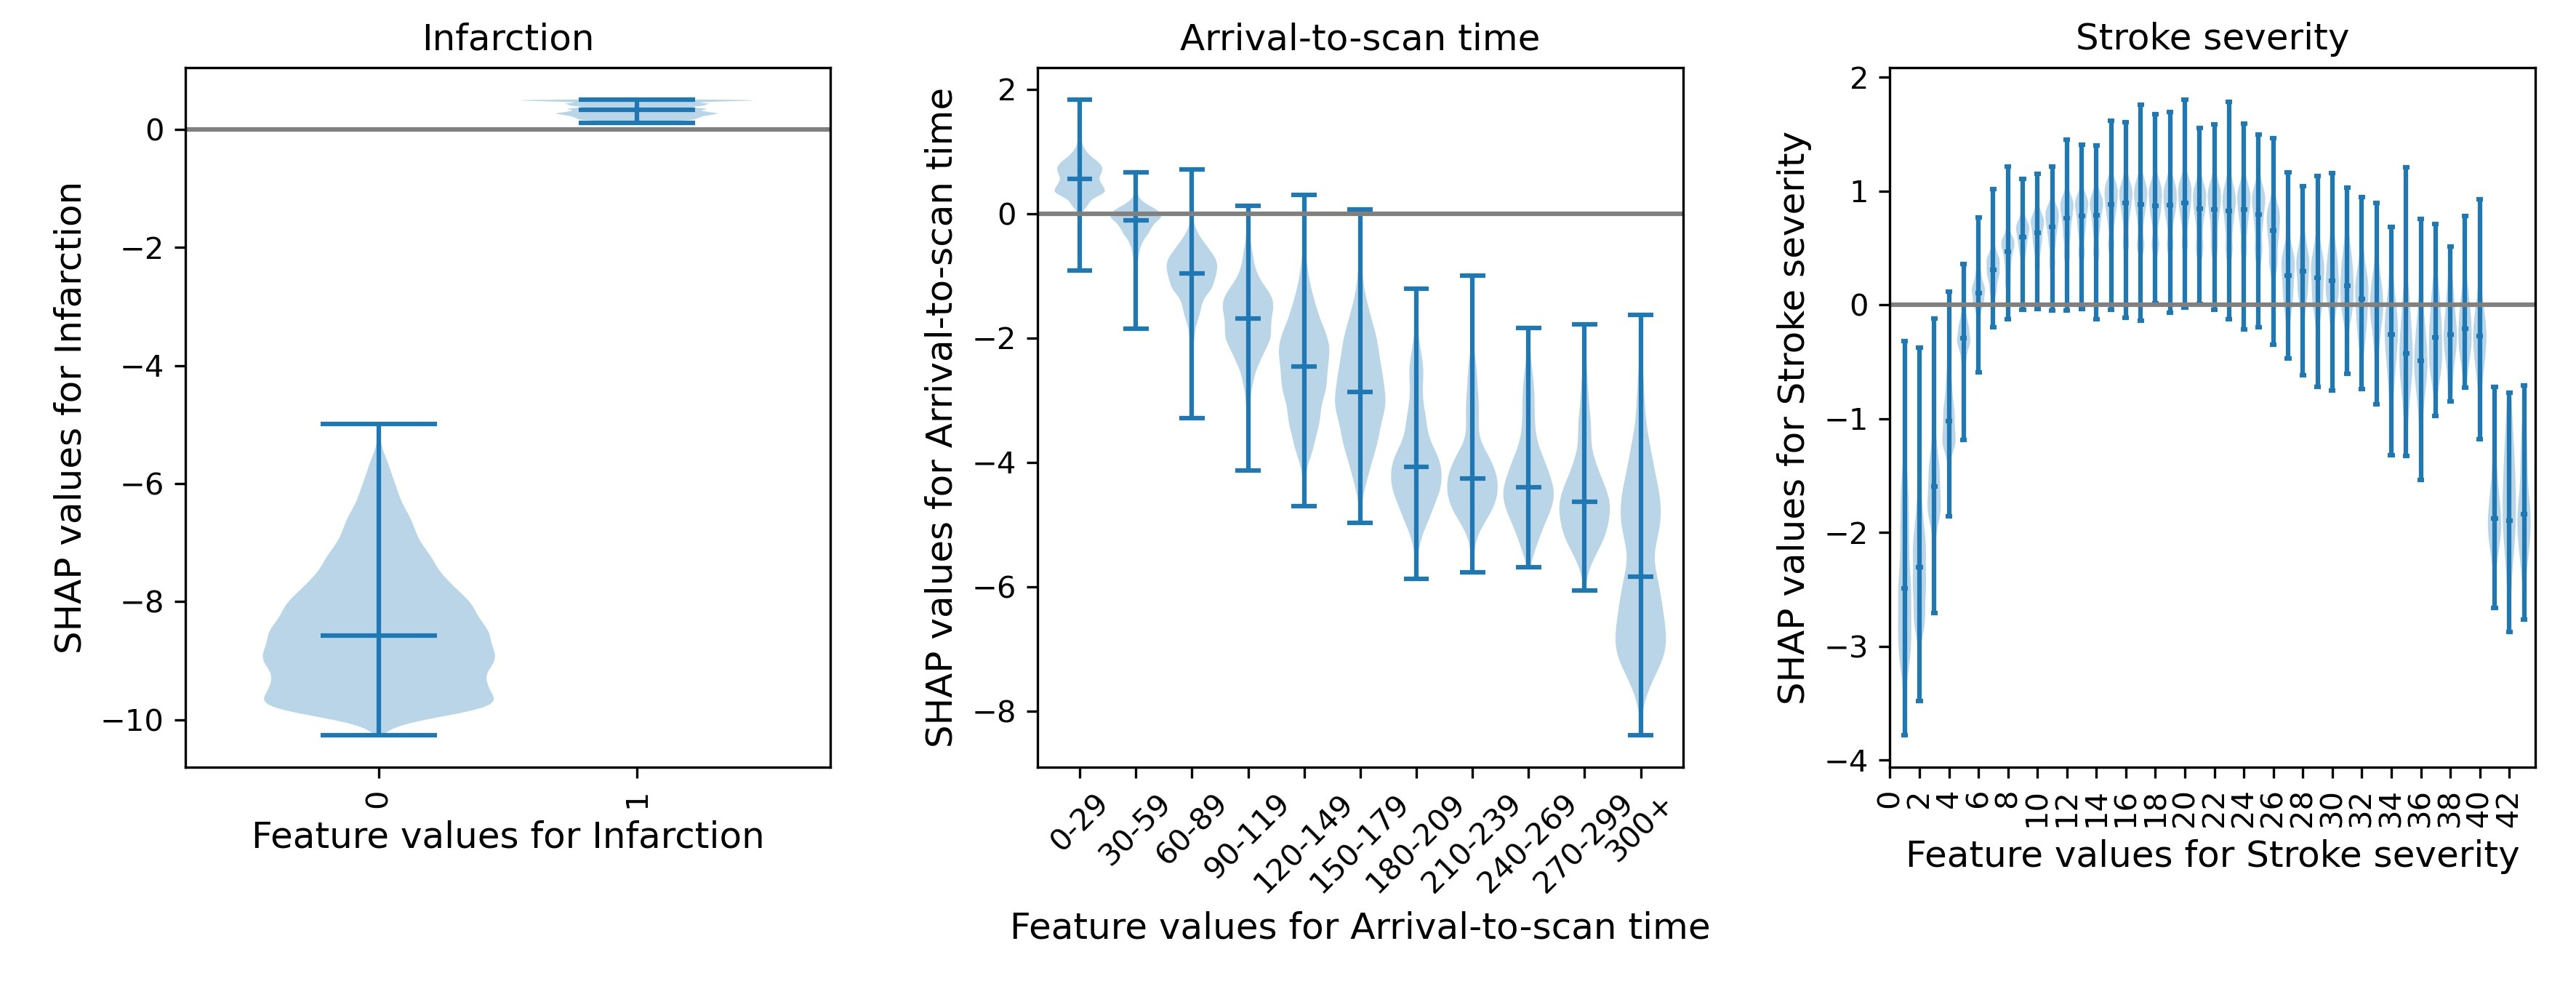
\includegraphics[width=1.0\textwidth]{./images/03d_xgb_10_features_thrombolysis_shap_violin_1.jpg}
\end{center}

\scriptsize
SHAP effects: \\
$\pm1$: Odds change $\pm3$ fold\\
$\pm2$: Odds change $\pm7$ fold\\
$\pm3$: Odds change $\pm20$ fold\\
$\pm4$: Odds change $\pm55$ fold\\
$\pm5$: Odds change $\pm150$ fold
\end{frame}
\begin{frame}
\frametitle{SHAP values for each feature - 2}
Note: SHAP values here are log odds. 
\begin{center}
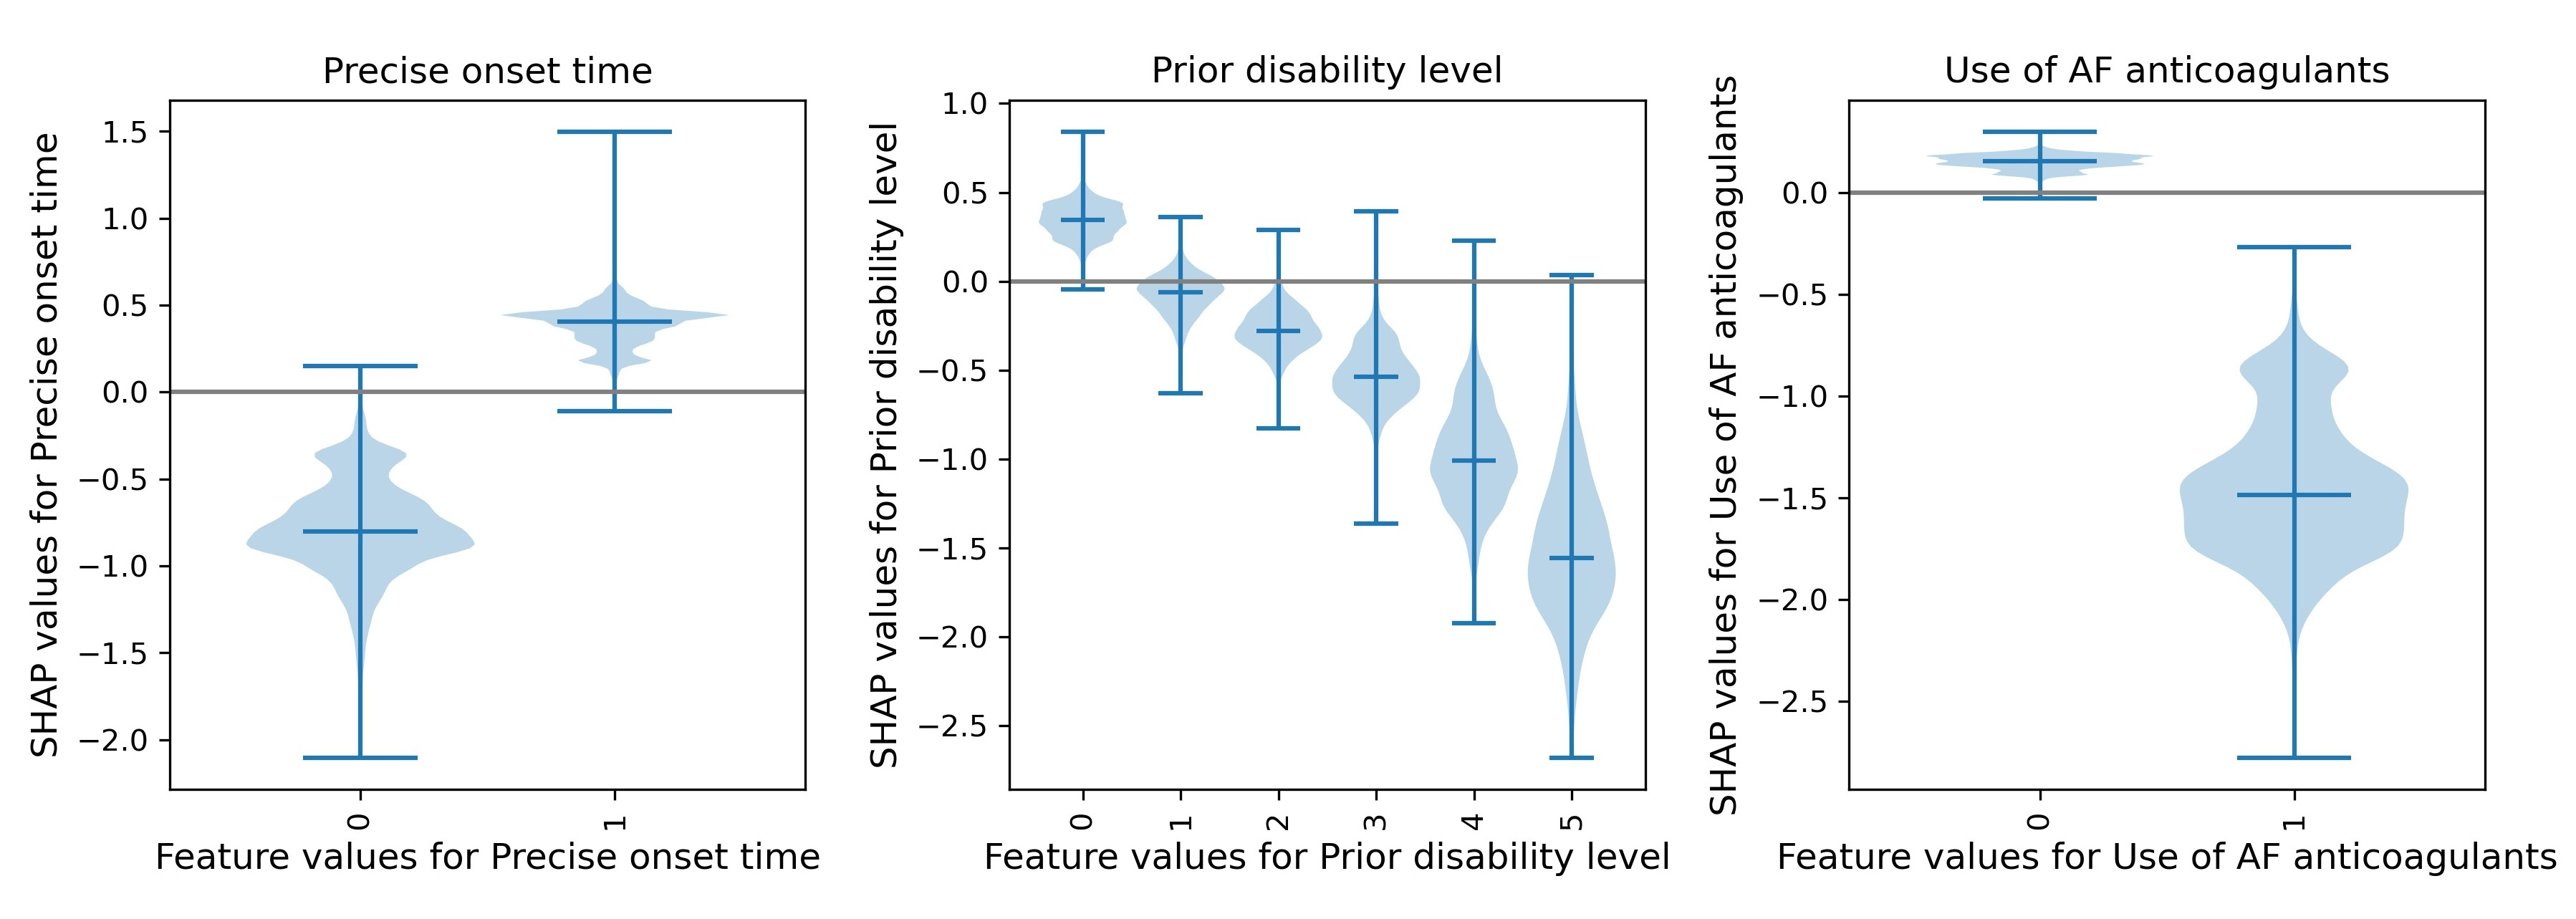
\includegraphics[width=1.0\textwidth]{./images/03d_xgb_10_features_thrombolysis_shap_violin_2.jpg}
\end{center}
\scriptsize
SHAP effects: \\
$\pm1$: Odds change $\pm3$ fold\\
$\pm2$: Odds change $\pm7$ fold\\
$\pm3$: Odds change $\pm20$ fold\\
$\pm4$: Odds change $\pm55$ fold\\
$\pm5$: Odds change $\pm150$ fold
\end{frame}
\begin{frame}
\frametitle{SHAP values for each feature - 3}
Note: SHAP values here are log odds. 
\begin{center}
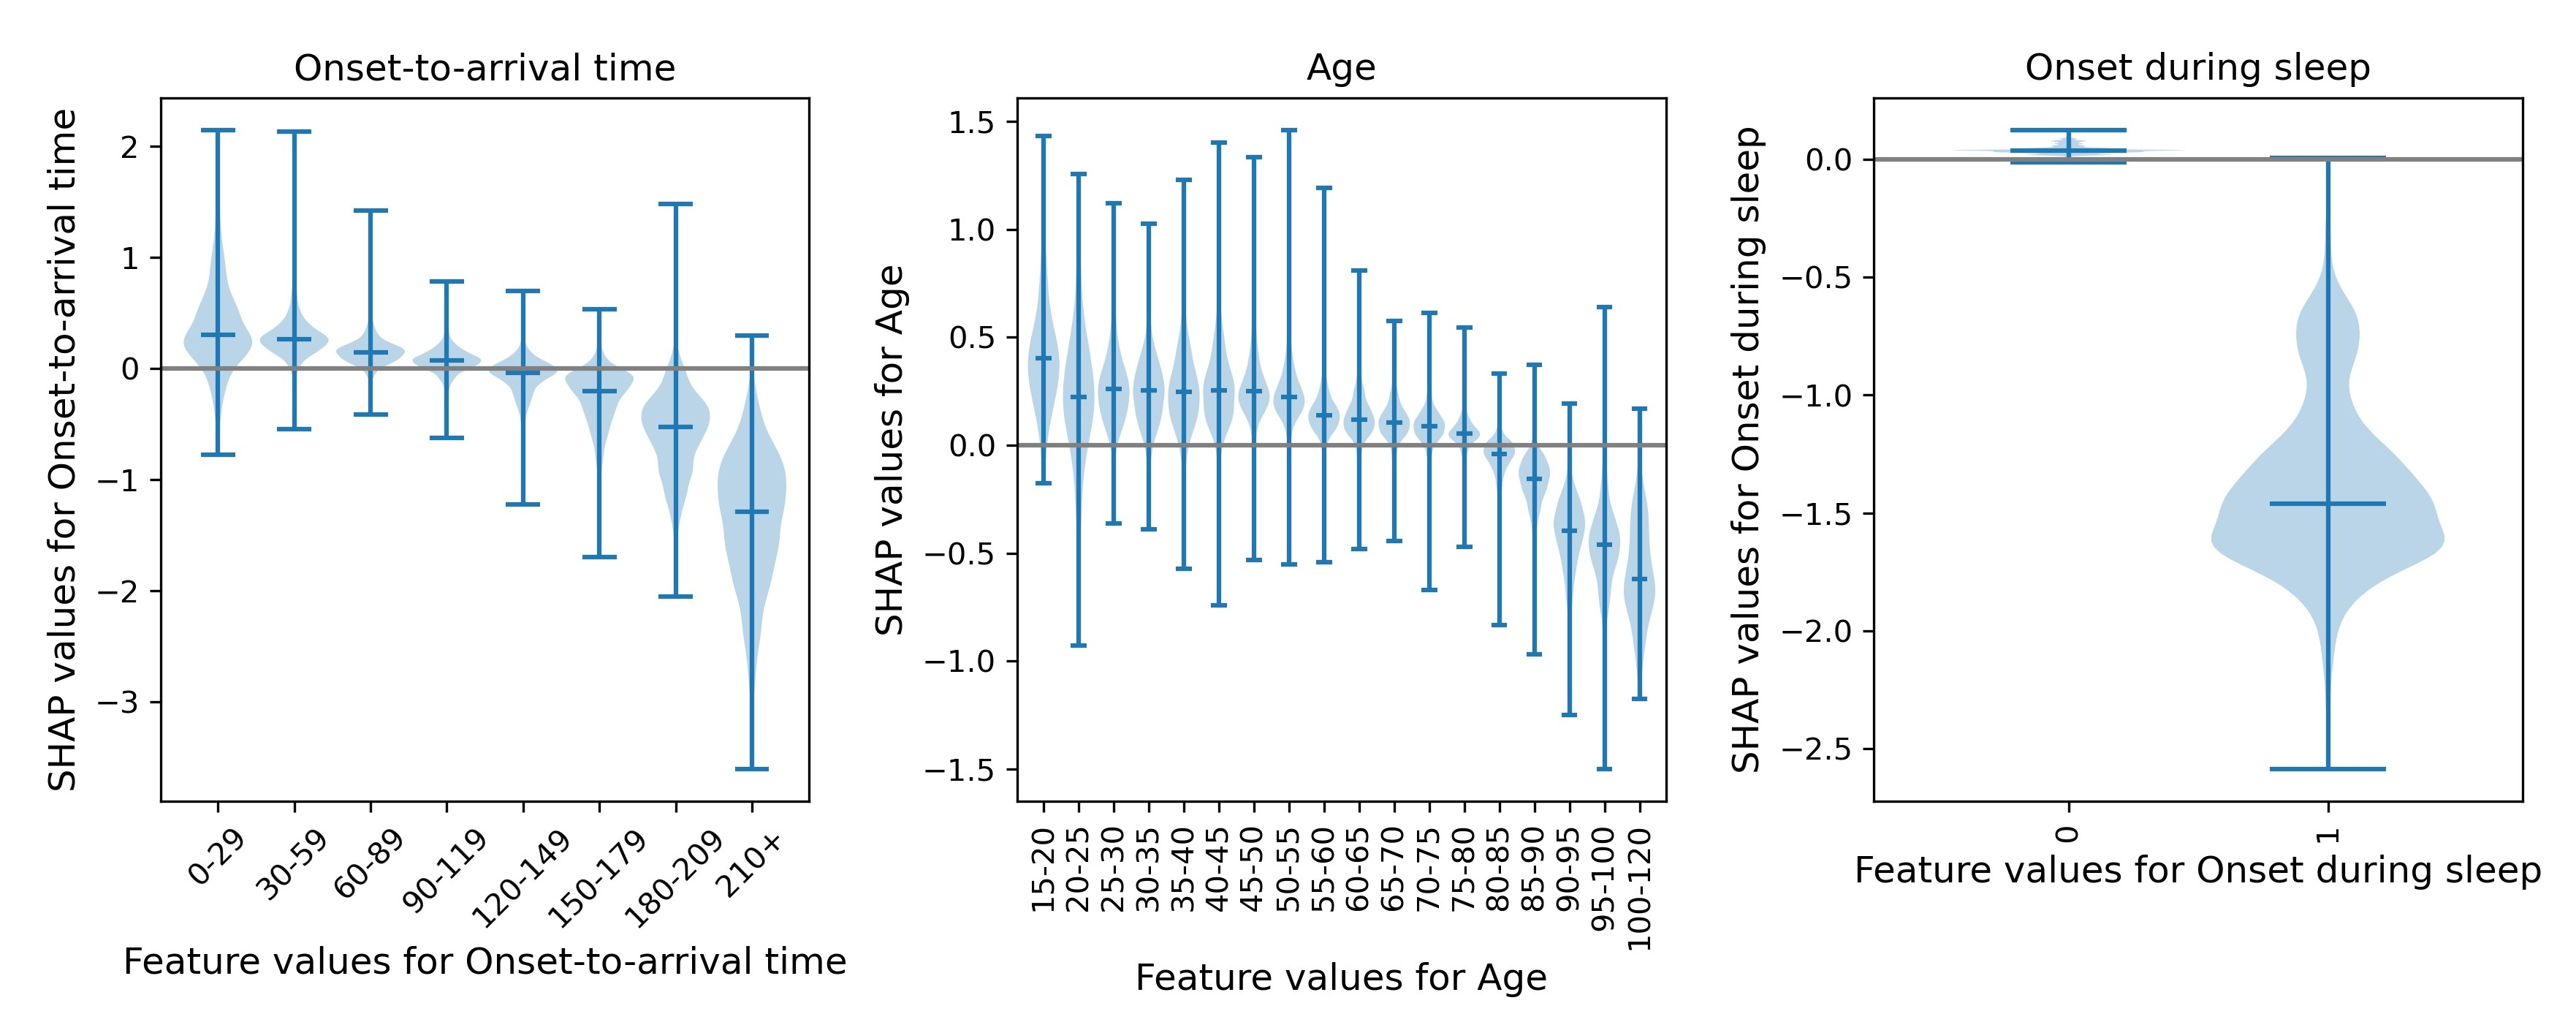
\includegraphics[width=1.0\textwidth]{./images/03d_xgb_10_features_thrombolysis_shap_violin_3.jpg}
\end{center}
\scriptsize
SHAP effects: \\
$\pm1$: Odds change $\pm3$ fold\\
$\pm2$: Odds change $\pm7$ fold\\
$\pm3$: Odds change $\pm20$ fold\\
$\pm4$: Odds change $\pm55$ fold\\
$\pm5$: Odds change $\pm150$ fold
\end{frame}
\begin{frame}
\frametitle{Isolating the effect of hospitals}
Note: SHAP values here are log odds. 
\begin{center}
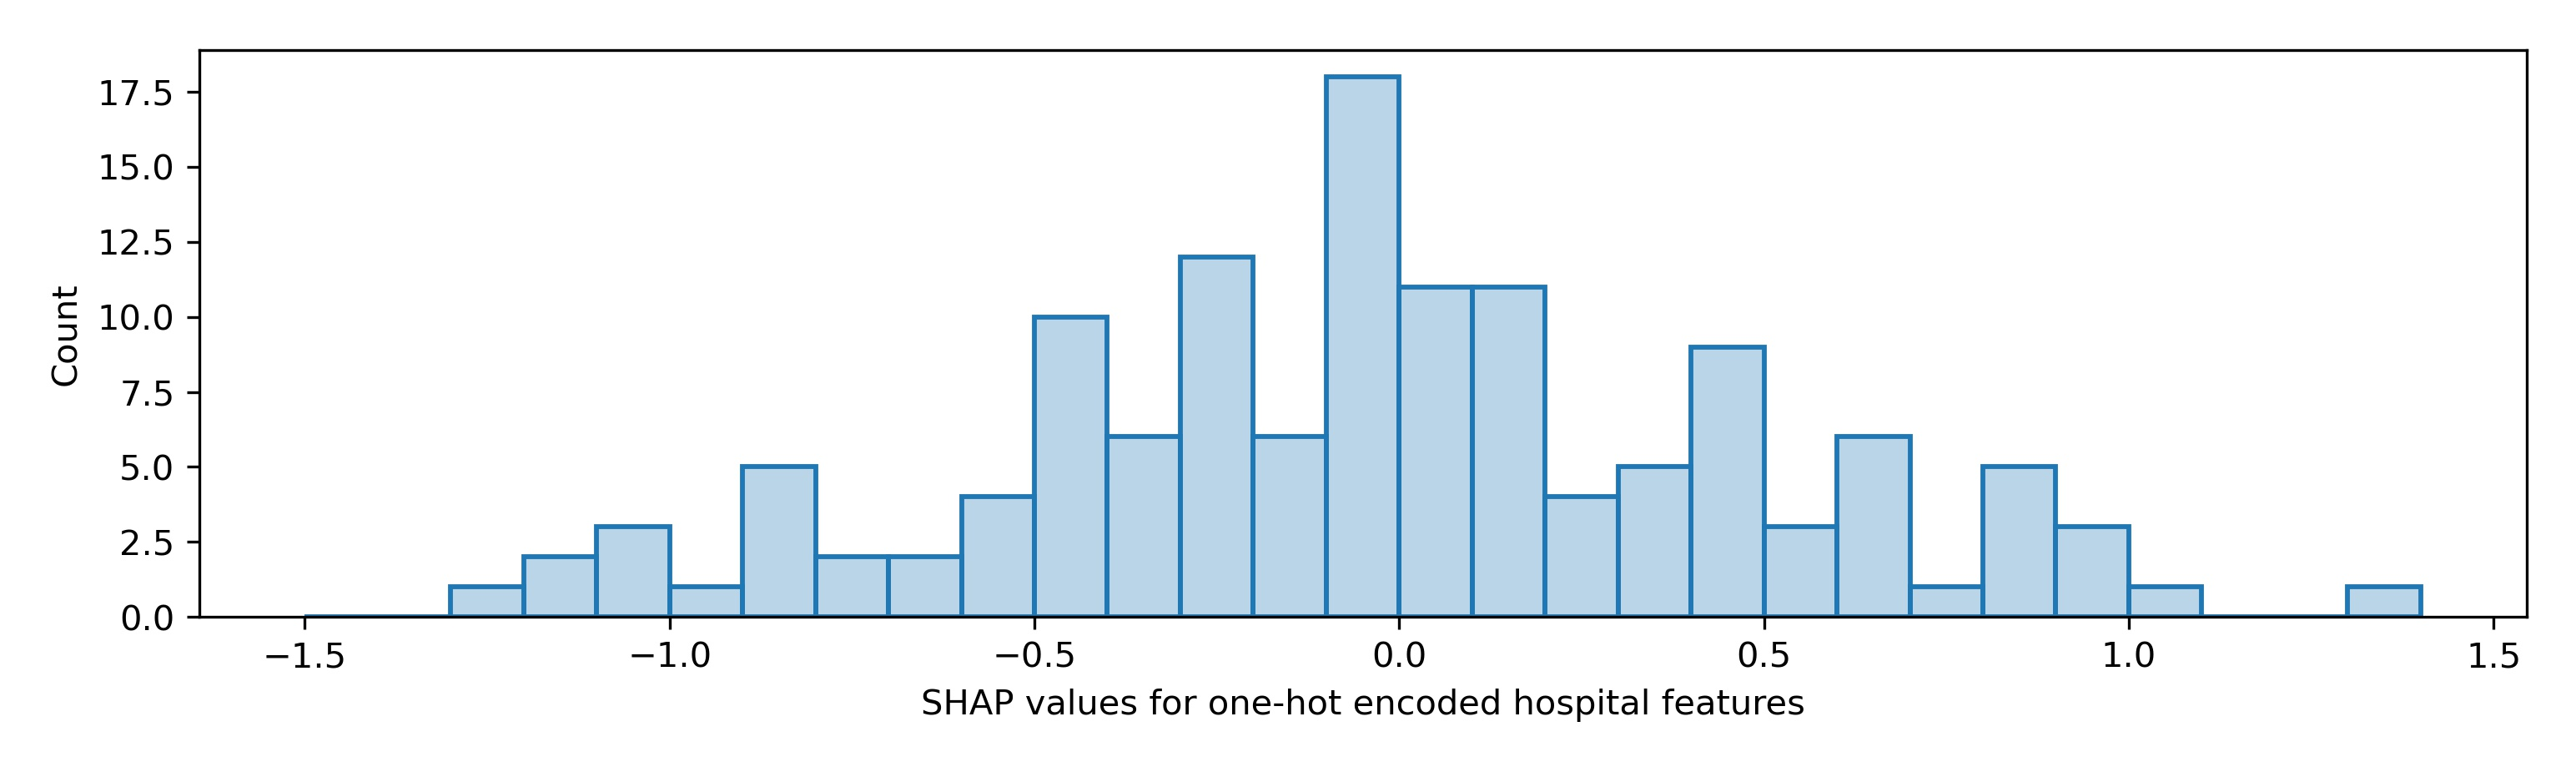
\includegraphics[width=1.0\textwidth]{./images/03d_xgb_10_features_hosp_shap_hist.jpg}
\end{center}
\scriptsize
SHAP effects: \\
$\pm1$: Odds change $\pm3$ fold\\
$\pm2$: Odds change $\pm7$ fold\\
$\pm3$: Odds change $\pm20$ fold\\
$\pm4$: Odds change $\pm55$ fold\\
$\pm5$: Odds change $\pm150$ fold
\end{frame}
\begin{frame}
\frametitle{What drives use of thrombolysis across all hospitals?}

The XGBoost/SHAP model revealed that the odds of receiving thrombolysis:

\vspace{2mm}

\begin{itemize}
    \setlength{\itemsep}{1.5mm}
    \item Reduced 20 fold over the first 100 minutes of arrival-to-scan time.
    \item Varied 30 fold depending on stroke severity.
    \item Reduced 3 fold with imprecise onset time.
    \item Fell 5 fold with increasing pre-stroke disability.
    \item Varied 15 fold between hospitals. 
    \item Fell 5 fold if the patient was taking anticoagulant medication.
    \item Was stable for the first two hours of arrival-to-onset time,and then fell 3 fold between two and four hours arrival-to-onset time
    \item Fell 2 fold between the age of 80 and 110.
    \item Fell 4 fold if onset was during sleep (these patients will also have the reduction due to imprecise onset time). 
\end{itemize}

\end{frame}
\begin{frame}
\frametitle{Regression of SHAP subgroups vs. hospital thrombolysis}

\begin{center}
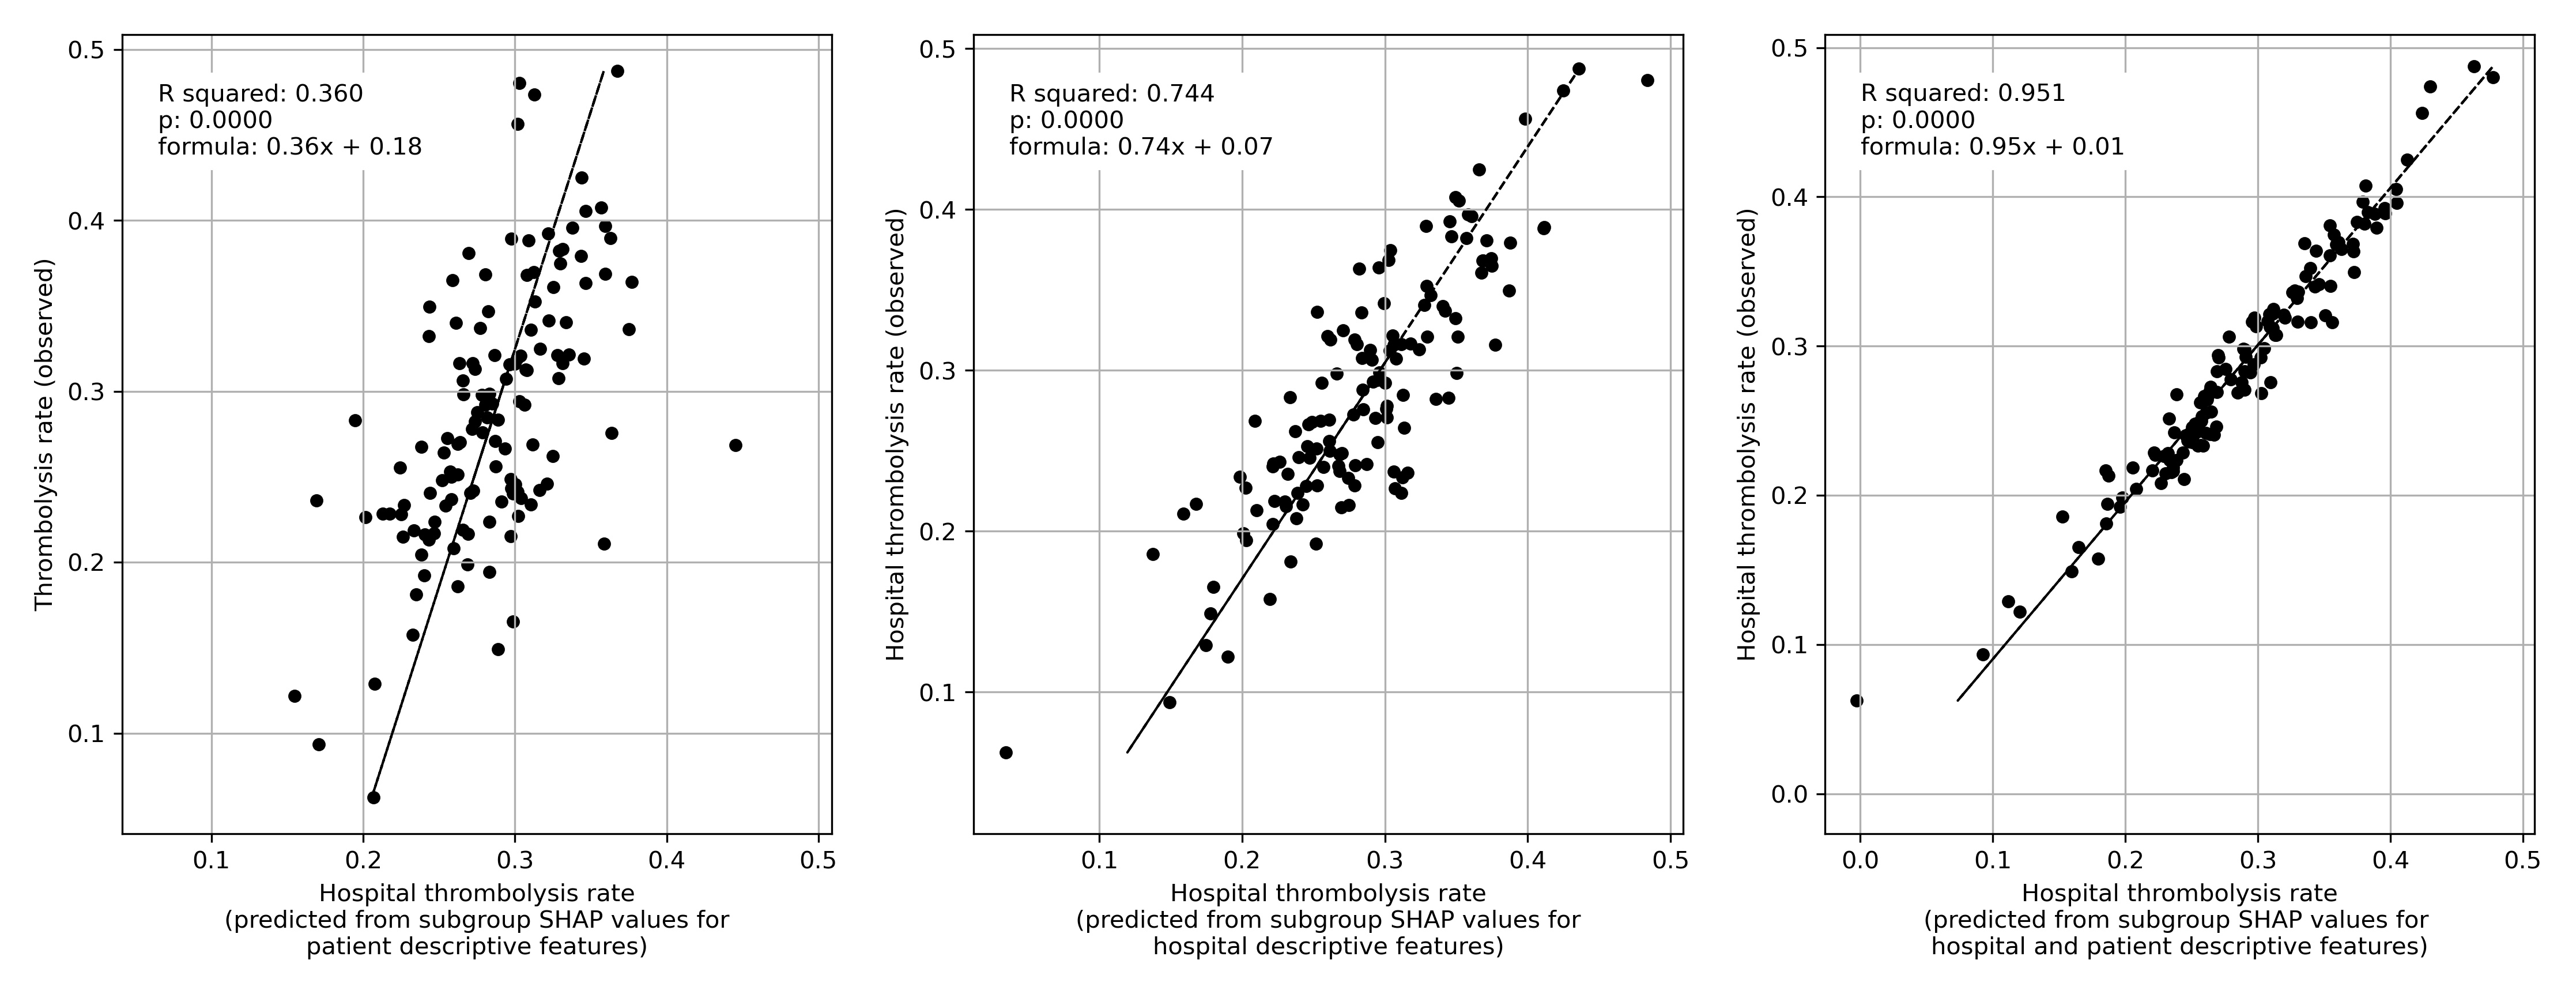
\includegraphics[width=0.95\textwidth]{./images/03e_xgb_10_features_multiple_regression_patient_hosptia_mean.jpg}
\end{center}

\scriptsize
\begin{itemize}
    \item Patient features (mean SHAP for each feature) alone explain 36\% of the variance in hospital thrombolysis use.
    \item Hospital features (men SHAP for hospital ID and arrival-to-scan time) alone explain 74\% of the variance in hospital thrombolysis use.
    \item Together, patient and hospital features explain 95\% of the variance in hospital thrombolysis use.
    \item Note: The sum of the patient-alone and hospital-one features = 110\%, suggesting we have a small amount of shared information between those groups.
\end{itemize}
 
\end{frame}
\begin{frame}
\frametitle{10k patient cohort}

\begin{itemize}

    
    \setlength{\itemsep}{4mm}
    \item In order to compare decision-making between hospitals, we selected 10k patients (stratified by hospital and thrombolysis use) to keep in a hold-back dataset.

    \item We trained model using the remaining 78,928 patients. 
    
    \item By passing all of the 10k patients (that were held back from the training process) through the fitted model, whilst setting the hospital attended feature to each hospital in turn, we predicted the thrombolysis rate for each hospital if all hospitals saw the same patients, revealing the variation in thrombolysis that is caused by the hospital, rather than by between-hospital variation in patient populations.
\end{itemize}
    
\end{frame}
\include{slides/055_shap_regression_10k}
\begin{frame}
\frametitle{Hospital SHAP predicts a hospital's predisposition to use thrombolysis}

\footnotesize Here we show the relationship of hospital SHAP with the hospital thrombolysis use for 1) the hospitals own patients, and 2) a common 10k cohort of patients.

\begin{center}
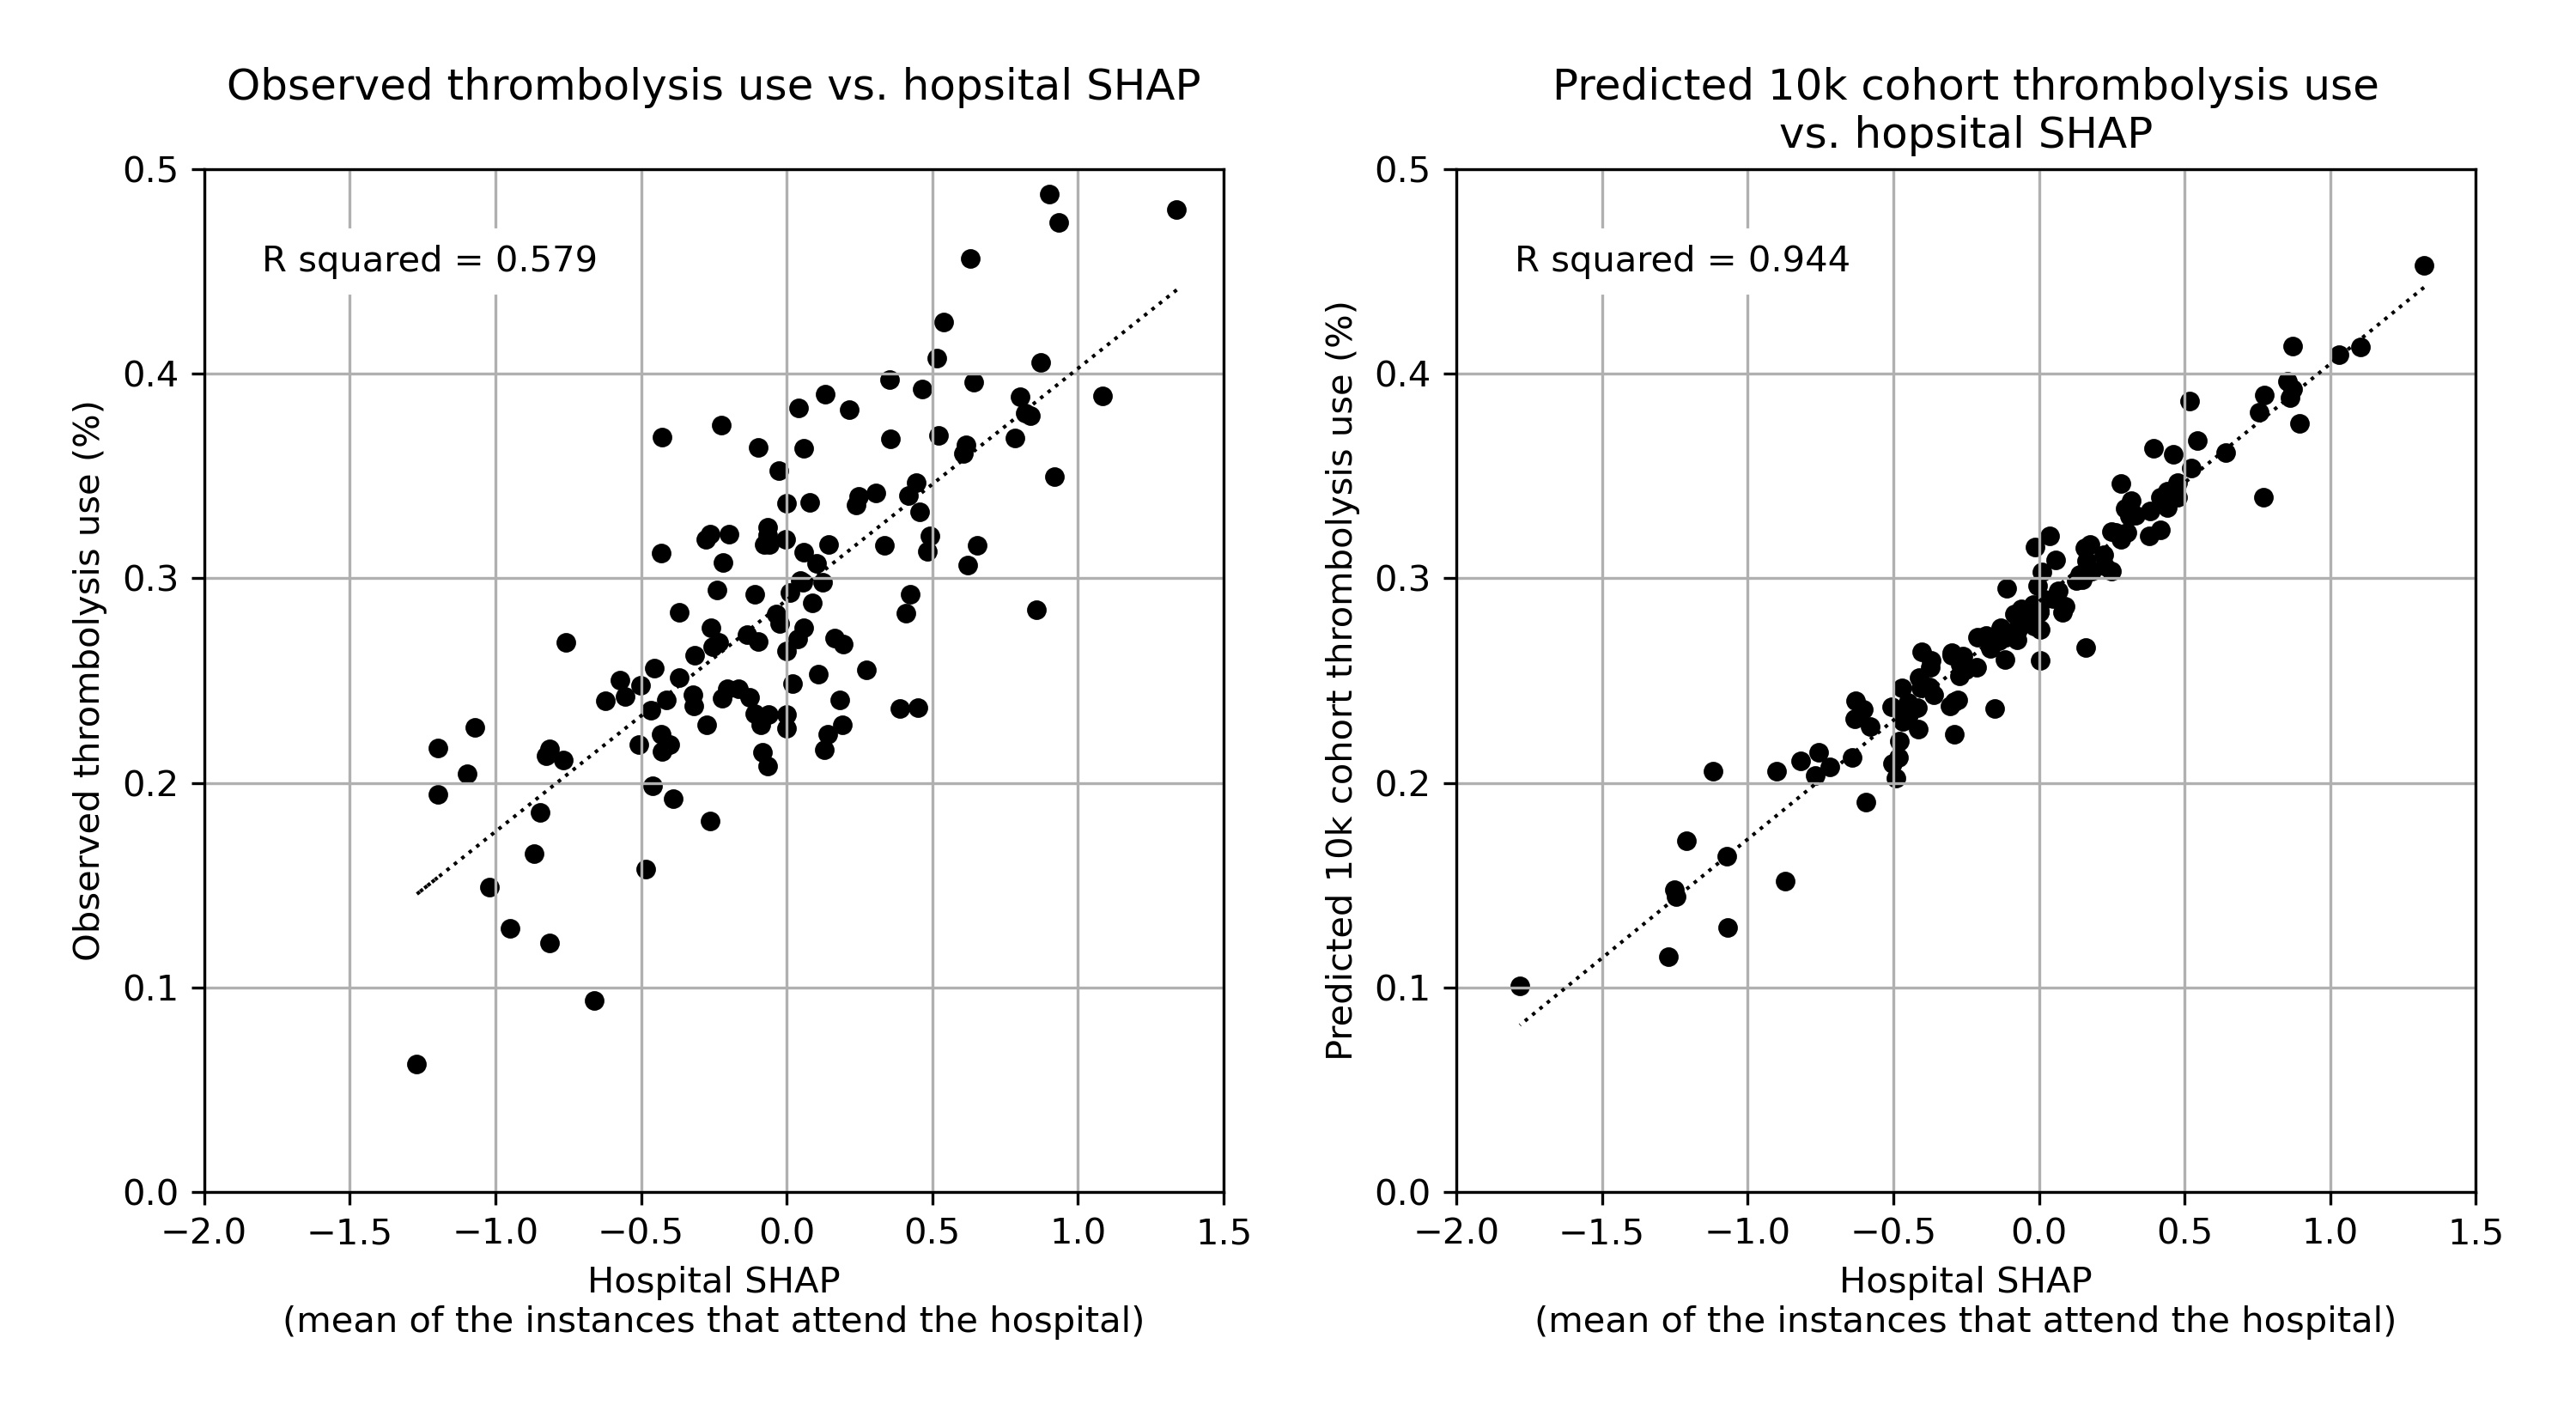
\includegraphics[width=1.0\textwidth]{./images/99_twin_correlation_scatter.jpg}
\end{center}
\end{frame}
\begin{frame}
\frametitle{How general effects may be modified by individual hospitals}

\begin{center}
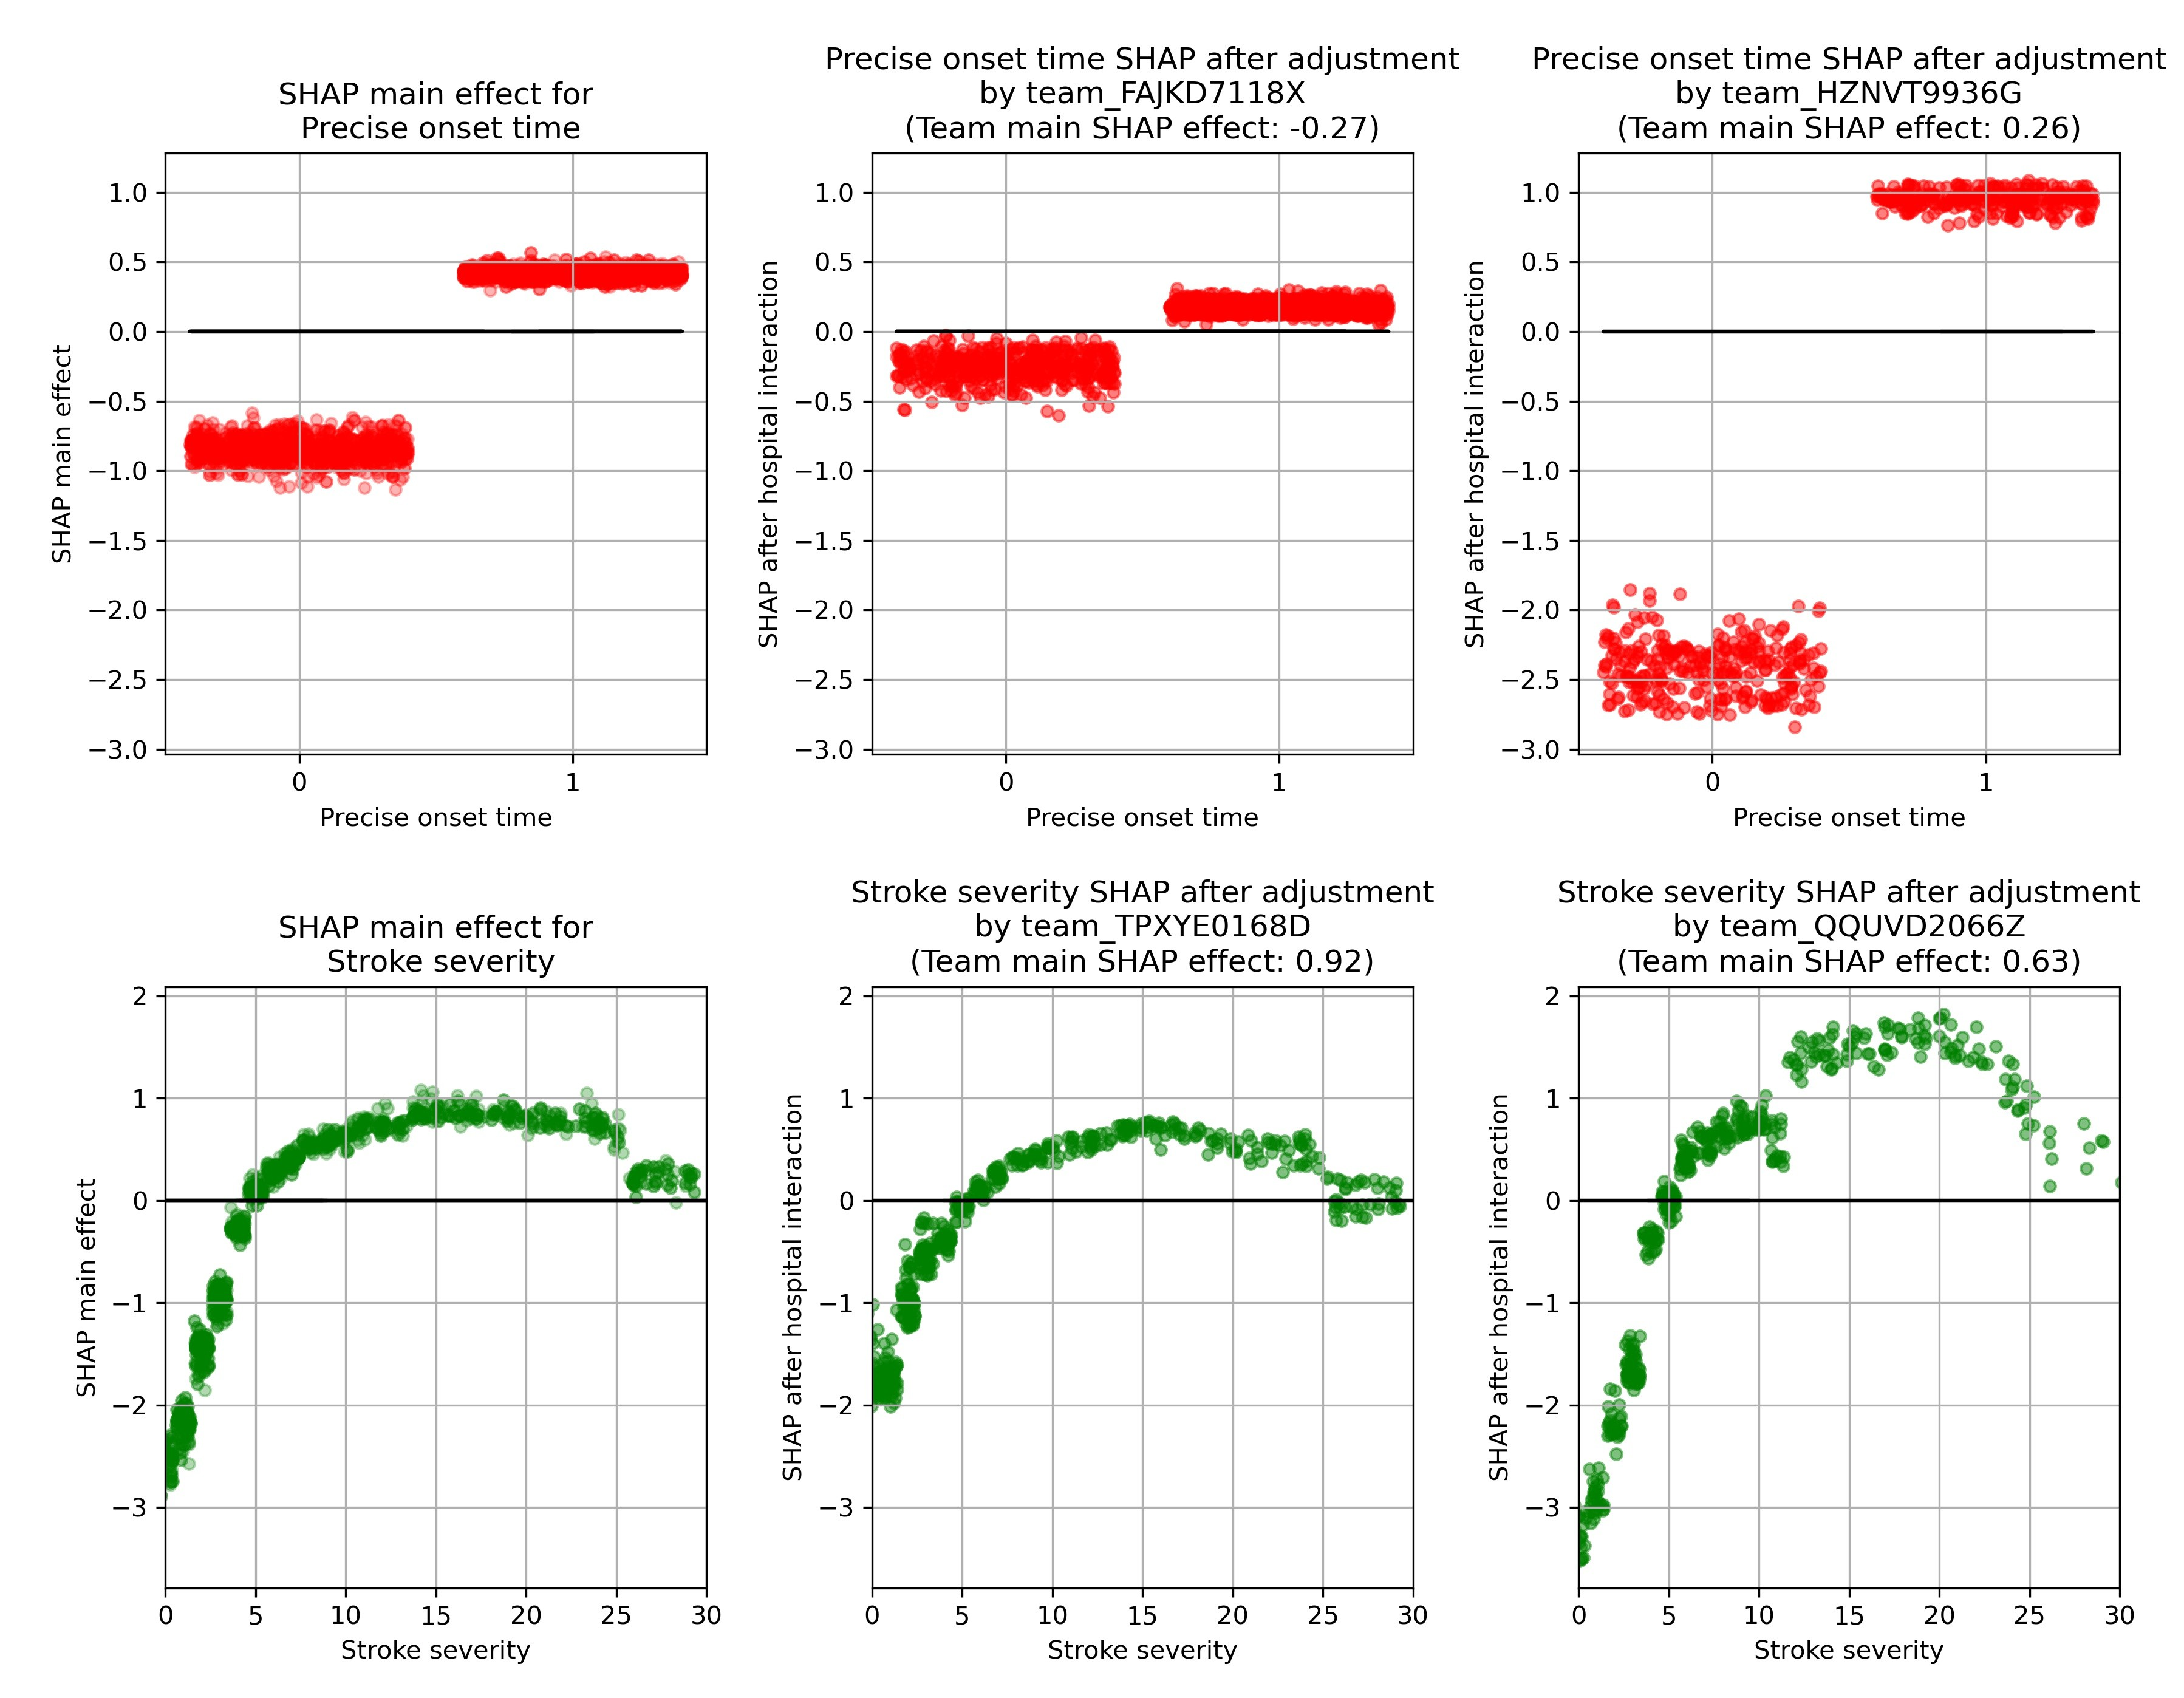
\includegraphics[width=0.88\textwidth]{./images/12aa_two_way_shap_adjustment.jpg}
\end{center}
\end{frame}
\begin{frame}
\frametitle{Thrombolysis in subgroups of patients (observed thrombolysis use in each team)}

\footnotesize The range of the predicted thrombolysis use across the 132 hospitals for subsets of patients attending each hopsital. 

\begin{center}
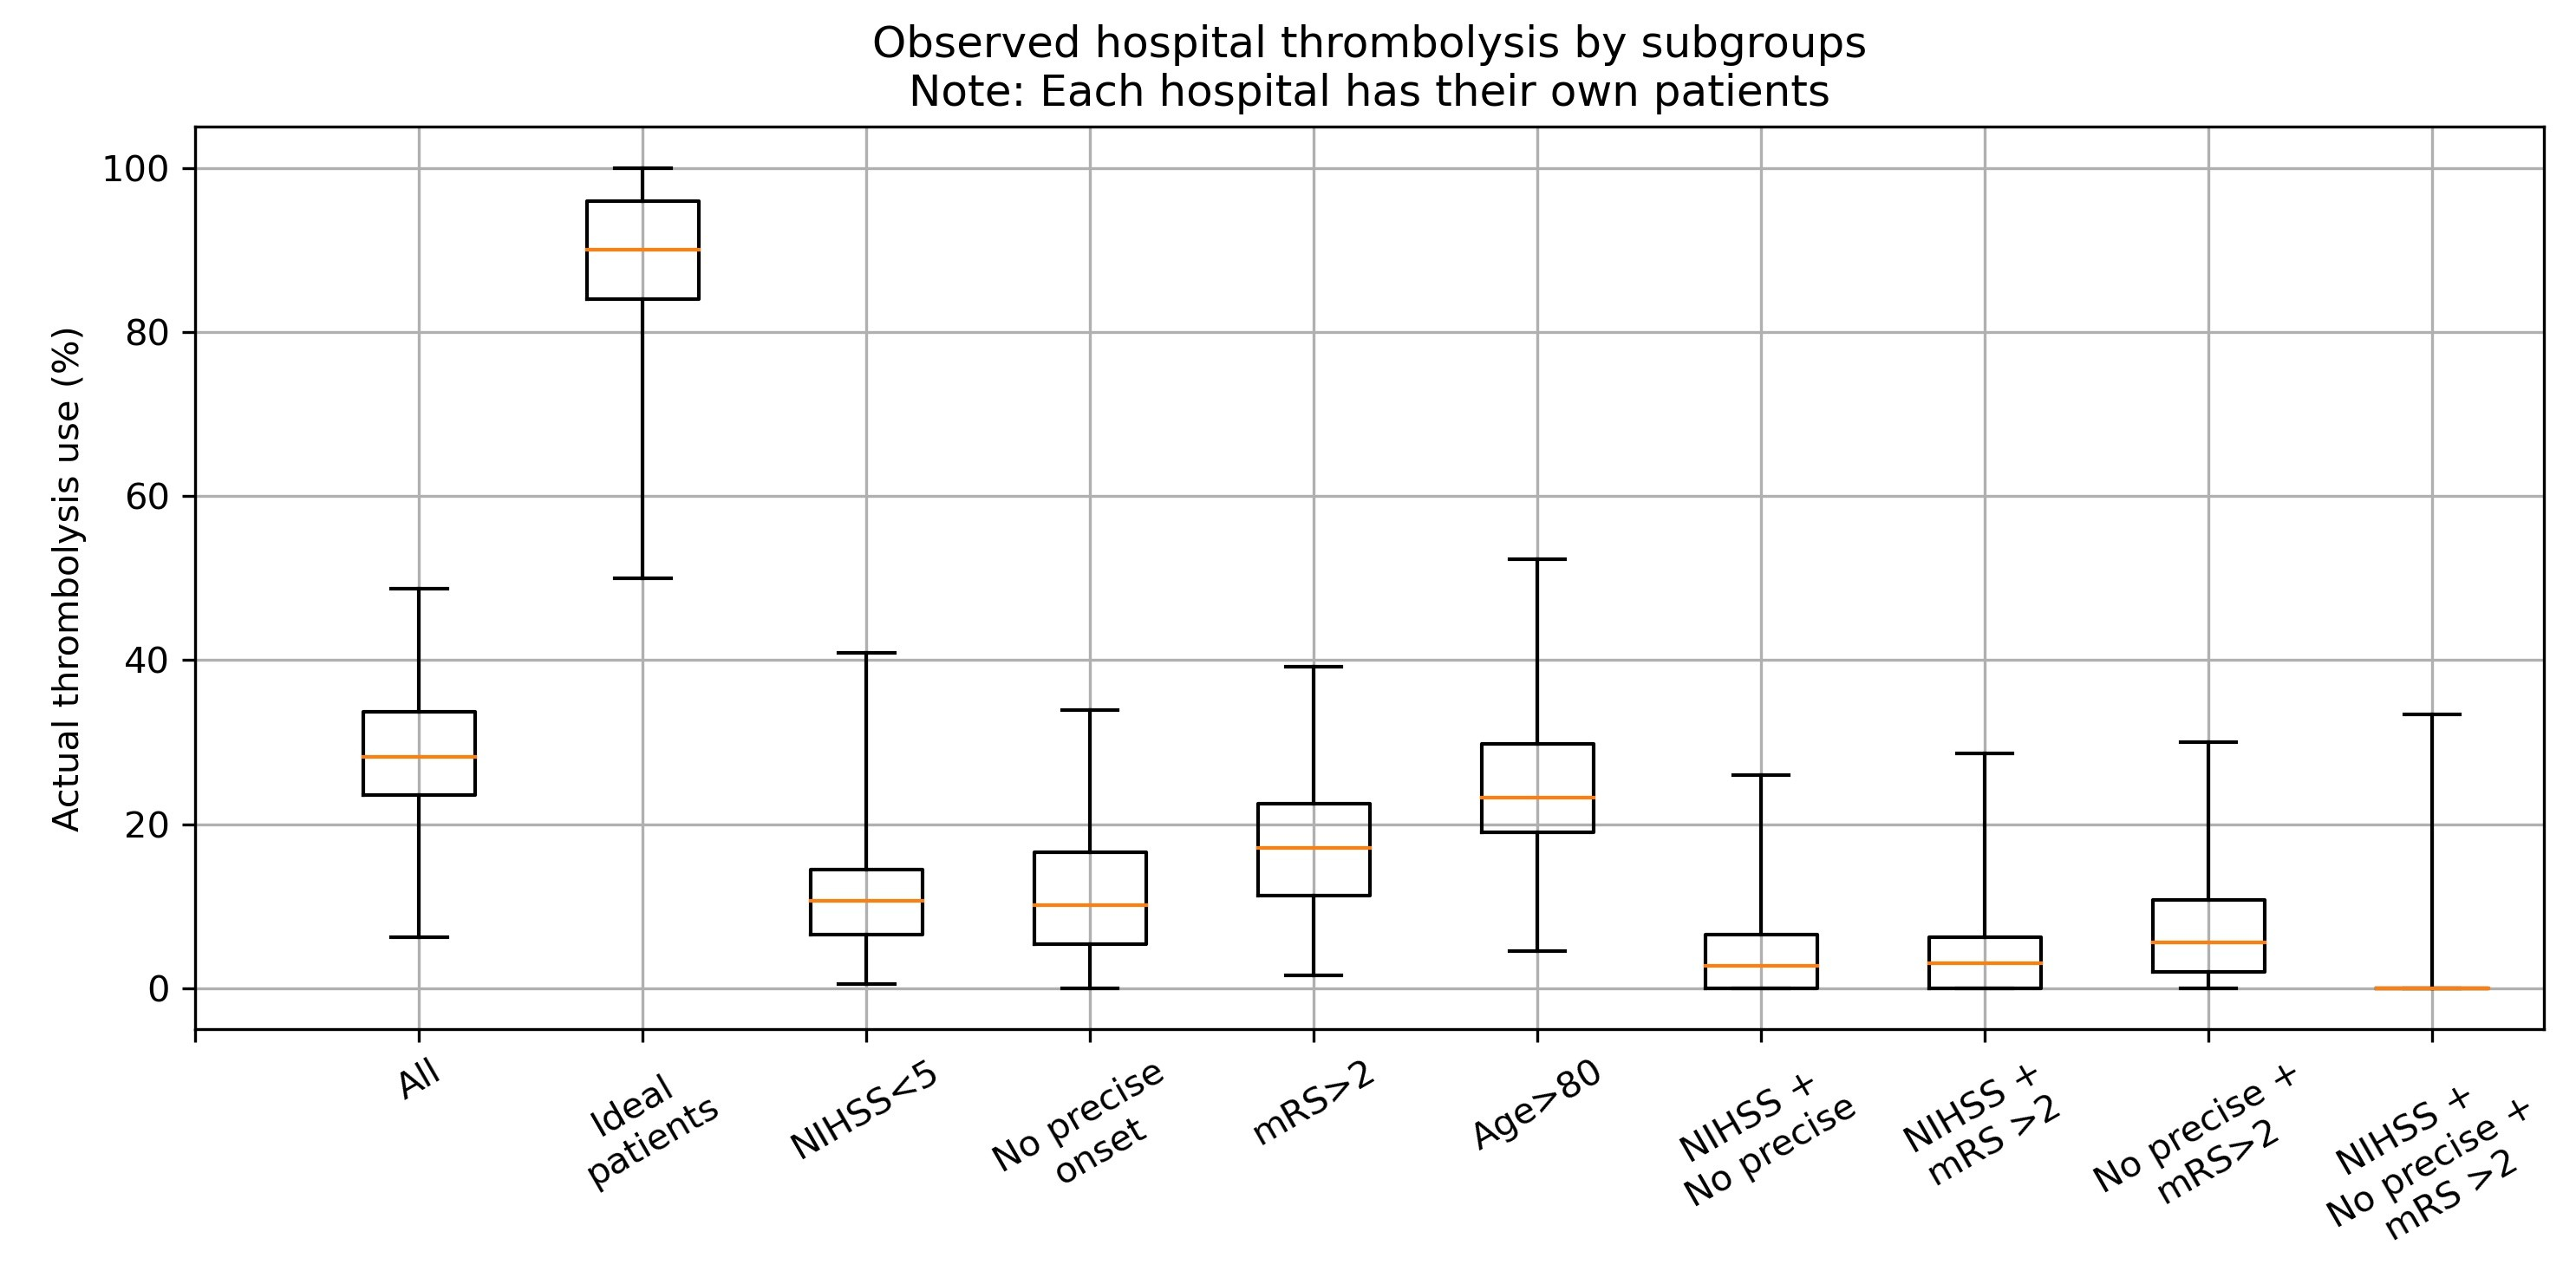
\includegraphics[width=0.83\textwidth]{./images/15b_actual_subgroup_violin.jpg}
\end{center}

\scriptsize An \emph{ideal patient} has: Stroke severity NIHSS in range 10-25, Arrival-to-scan time \textless{} 20 minutes, Stroke type = infarction, Precise onset time = True, Prior disability level (mRS) = 0, No use of AF anticoagulants, Onset-to-arrival time \textless{} 90 minutes, Age \textless{80 years}, Onset during sleep = False
\end{frame}
\begin{frame}
\frametitle{Thrombolysis in subgroups of patients (observed thrombolysis use in each team)}

\footnotesize The range of the predicted thrombolysis use across the 132 hospitals for subsets of patients attending each hopsital. 

\begin{center}
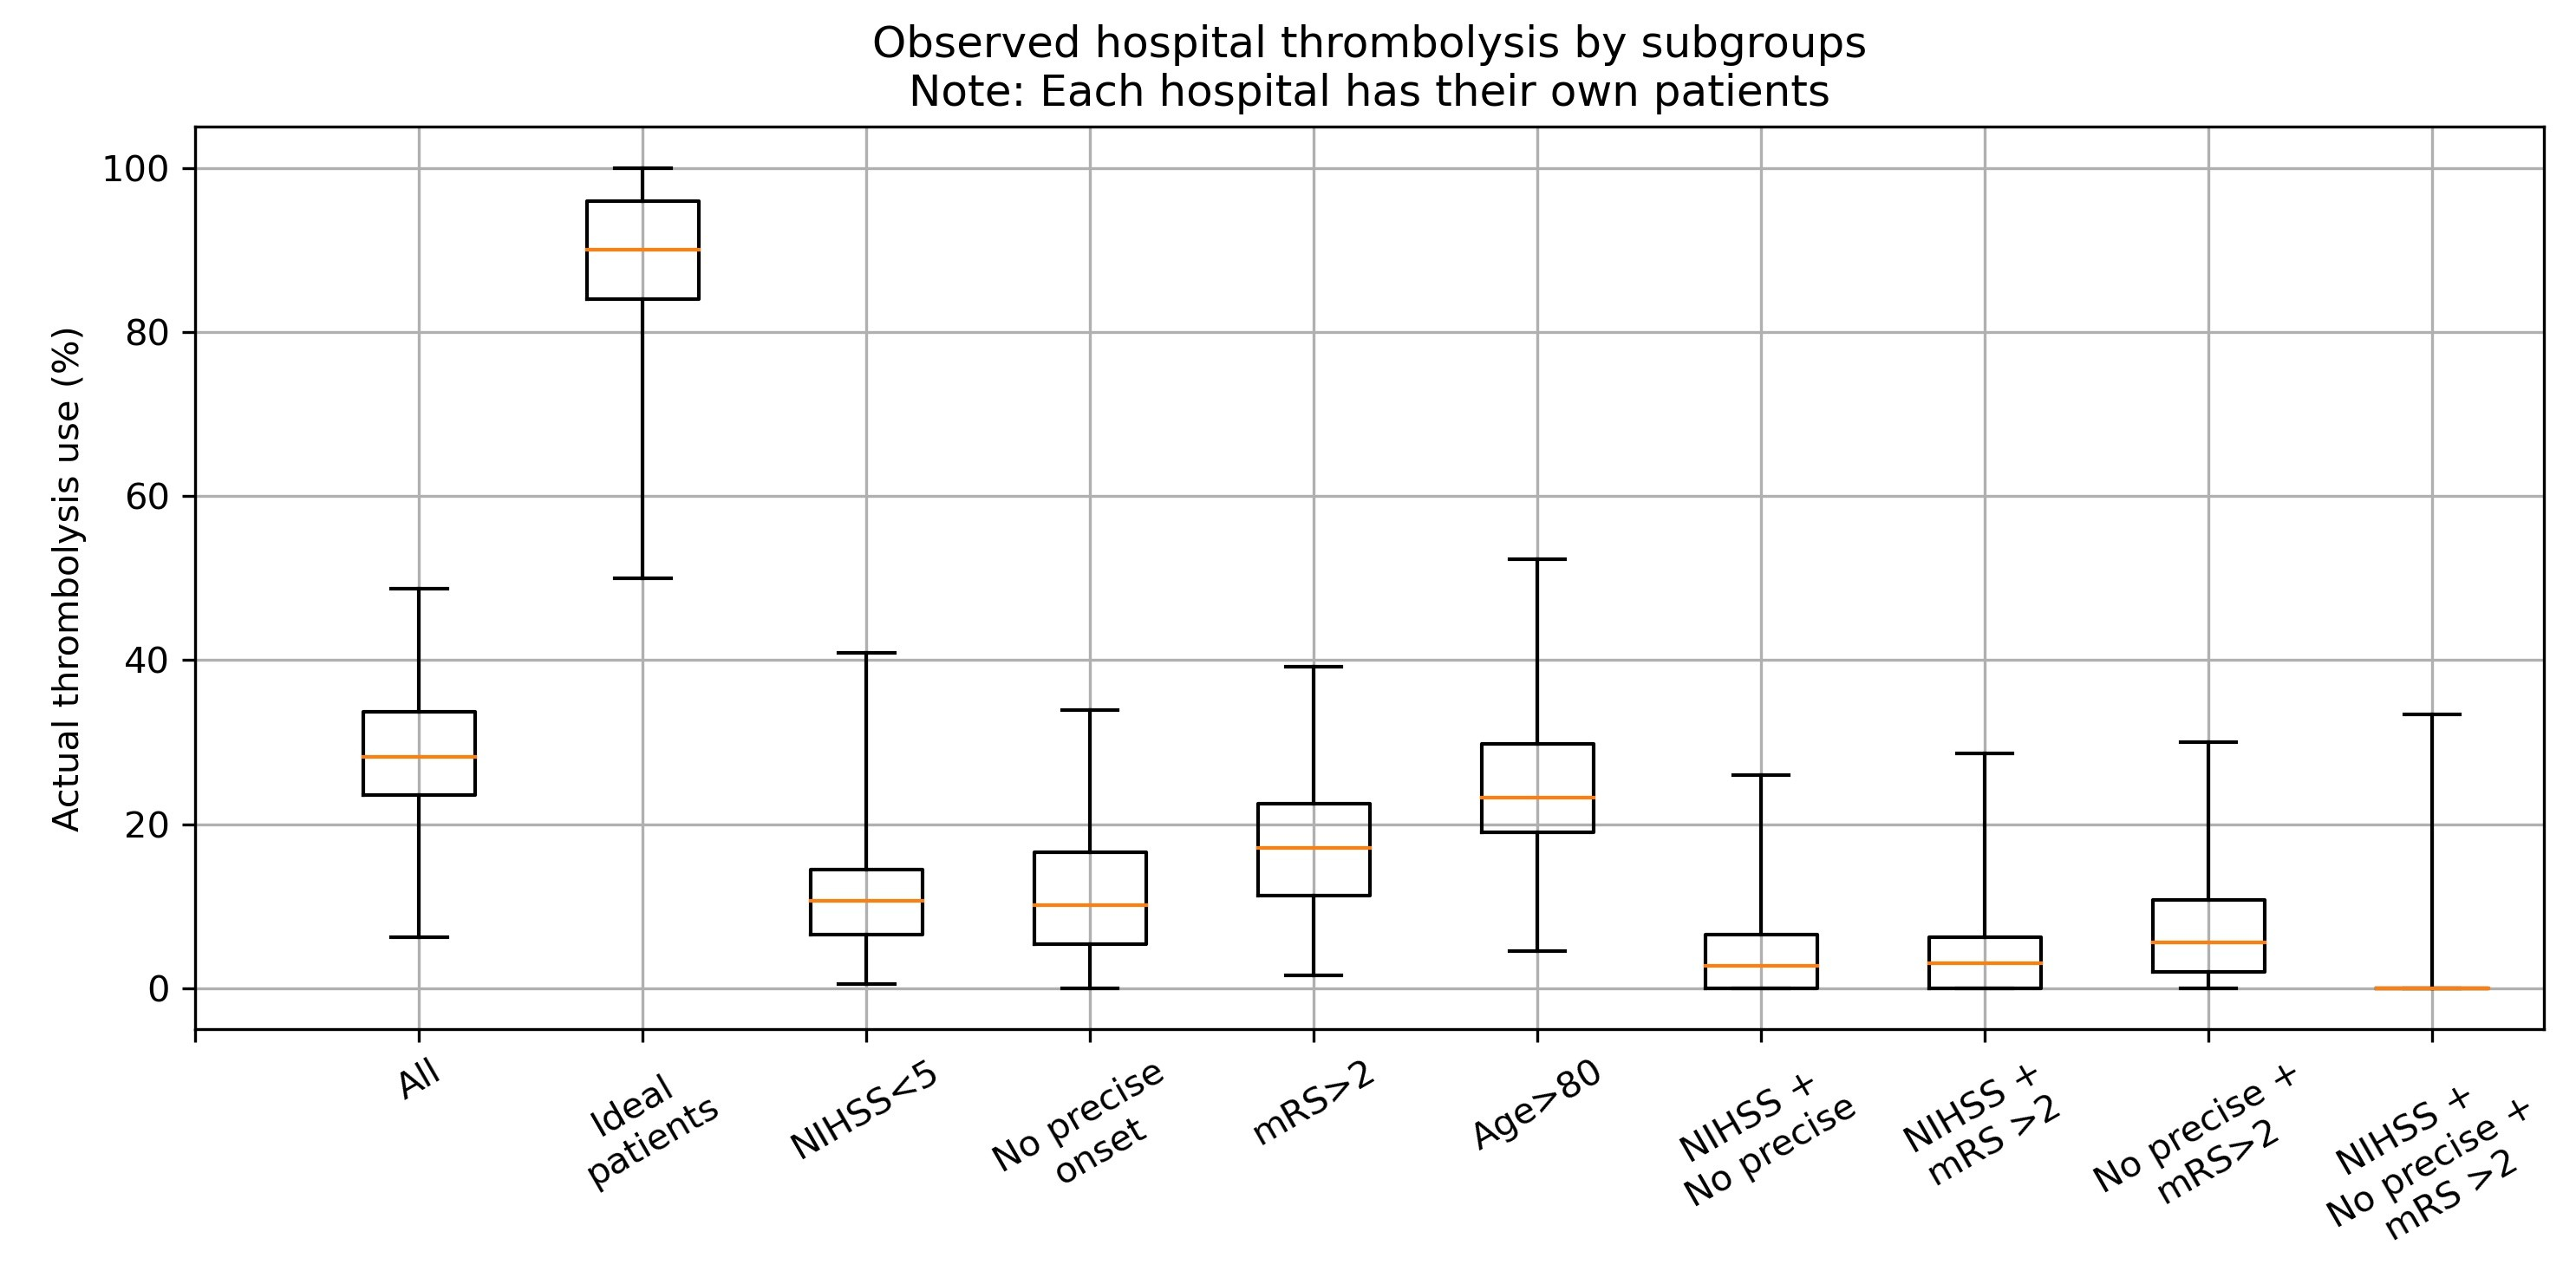
\includegraphics[width=0.83\textwidth]{./images/15b_actual_subgroup_violin.jpg}
\end{center}

\scriptsize An \emph{ideal patient} has: Stroke severity NIHSS in range 10-25, Arrival-to-scan time \textless{} 20 minutes, Stroke type = infarction, Precise onset time = True, Prior disability level (mRS) = 0, No use of AF anticoagulants, Onset-to-arrival time \textless{} 90 minutes, Age \textless{80 years}, Onset during sleep = False
\end{frame}
\begin{frame}
\frametitle{Thrombolysis in subgroups of patients (observed use in each hospitals own patients)}

    \begin{center}
    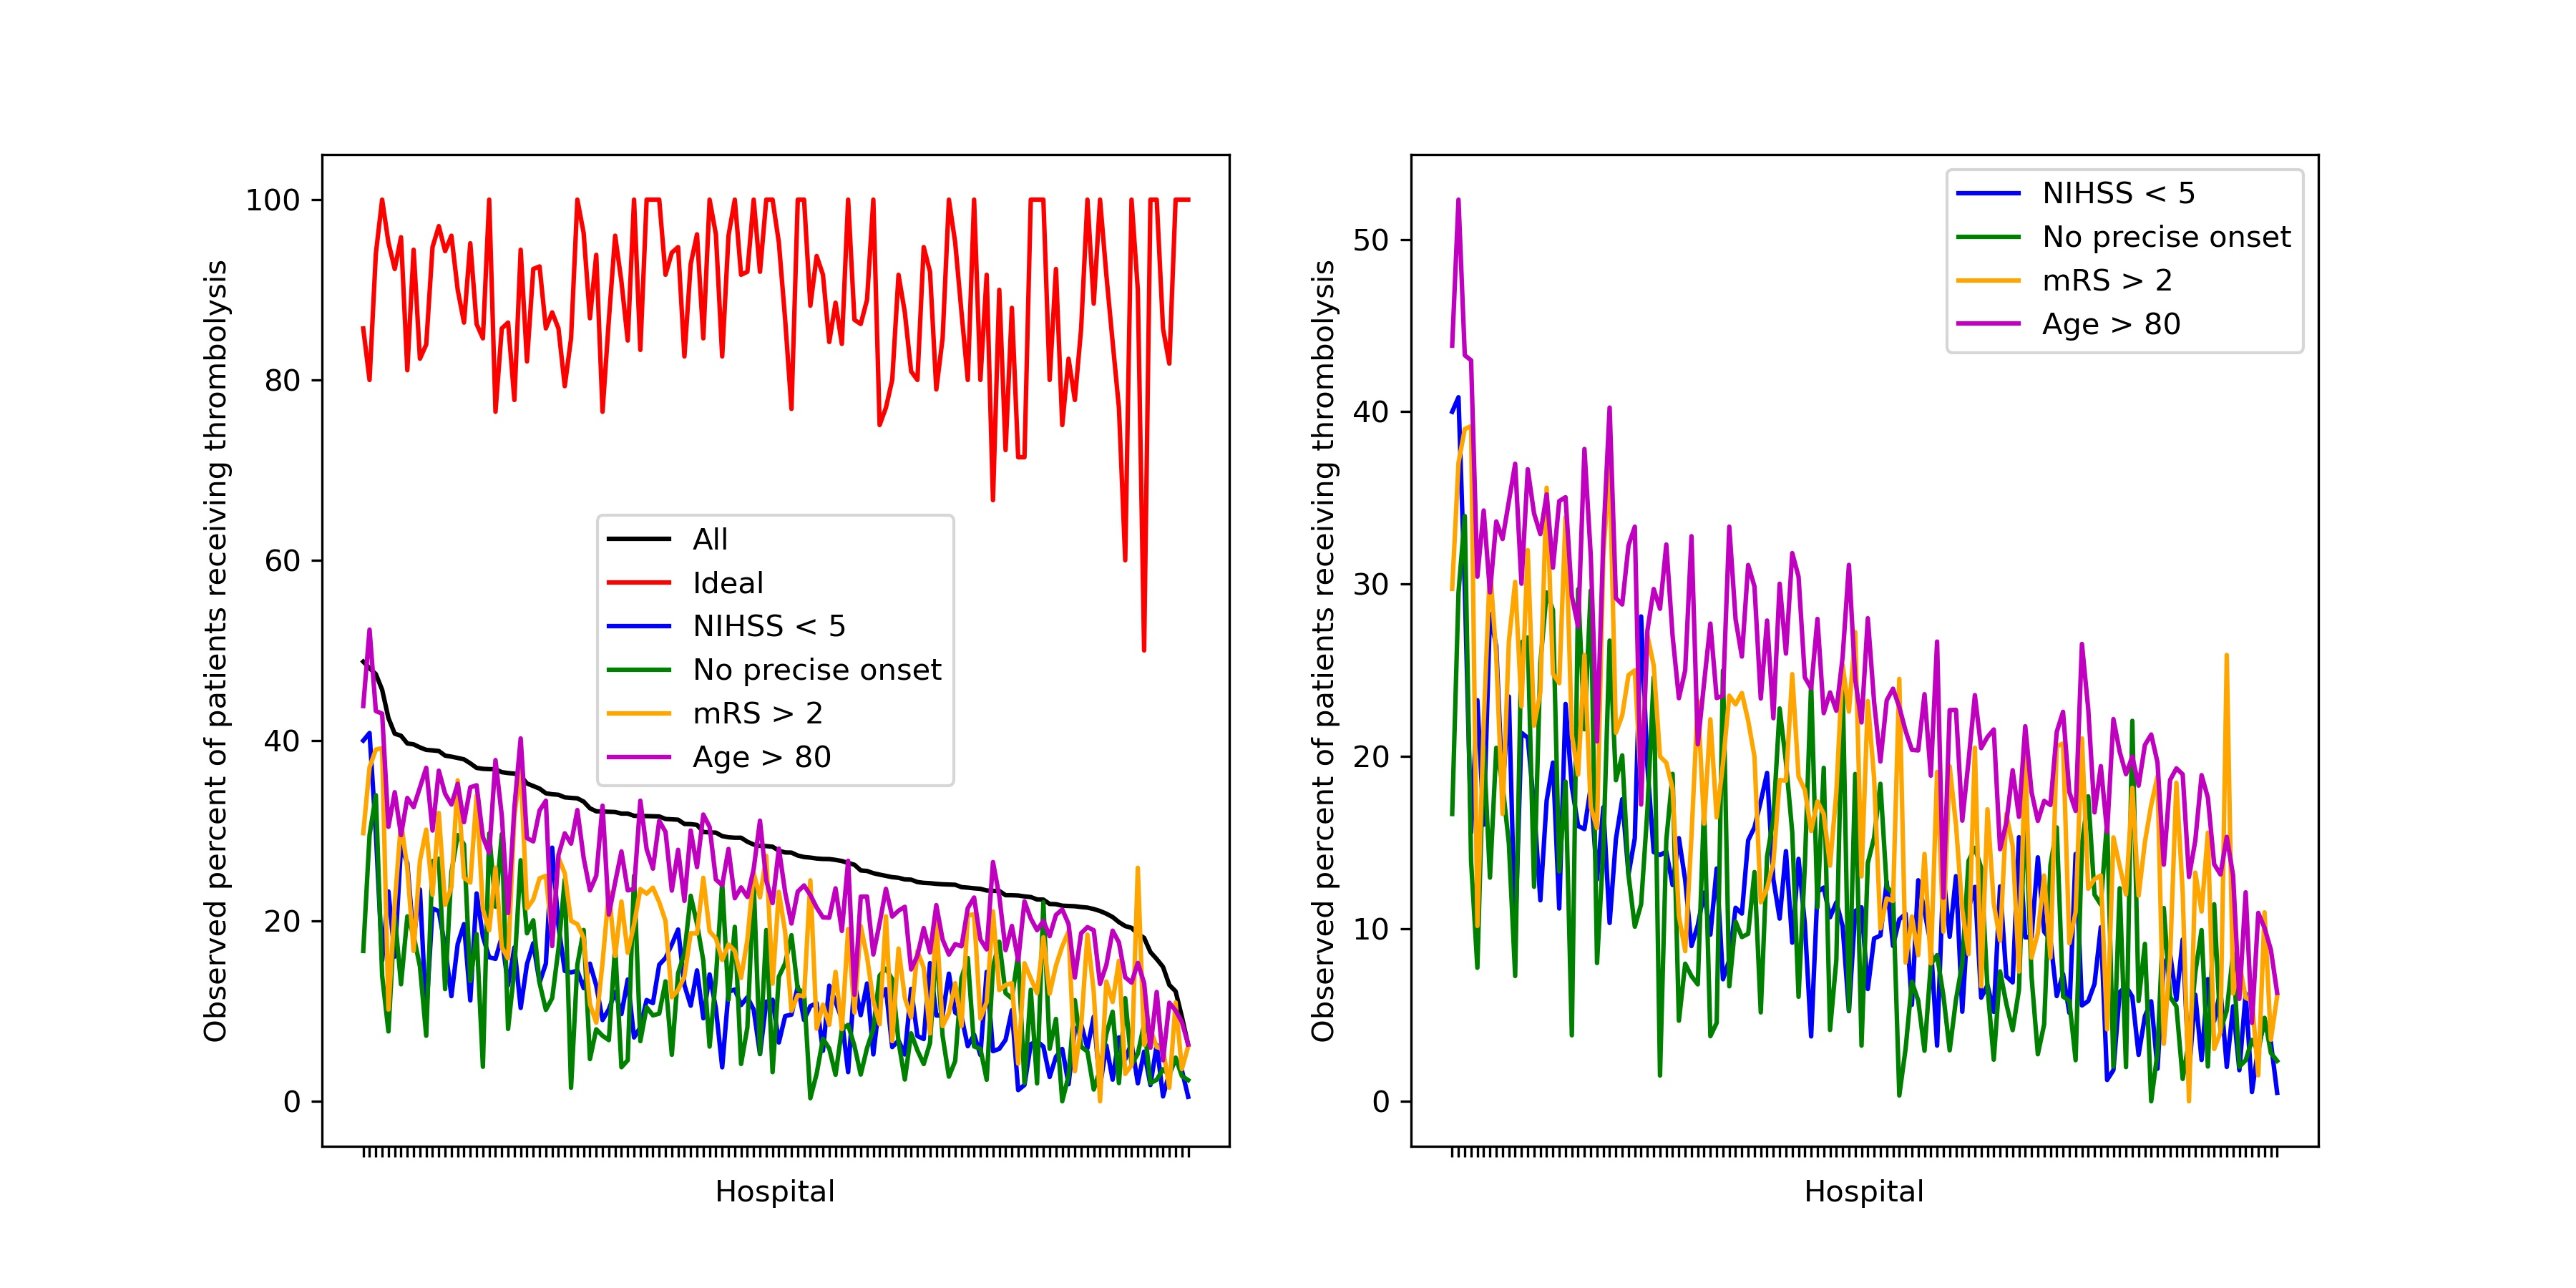
\includegraphics[width=0.95\textwidth]{./images/15a_actual_subgroup.jpg}
    \end{center}

\footnotesize Note: Subgroups, other than \emph{ideal patients}, tend to track each other, but with more noise than predicted thrombolysis use. 

\end{frame}

\begin{frame}
\frametitle{Thrombolysis in subgroups of patients (predicted use in a common 10k cohort at each hospital)}

    \begin{center}
    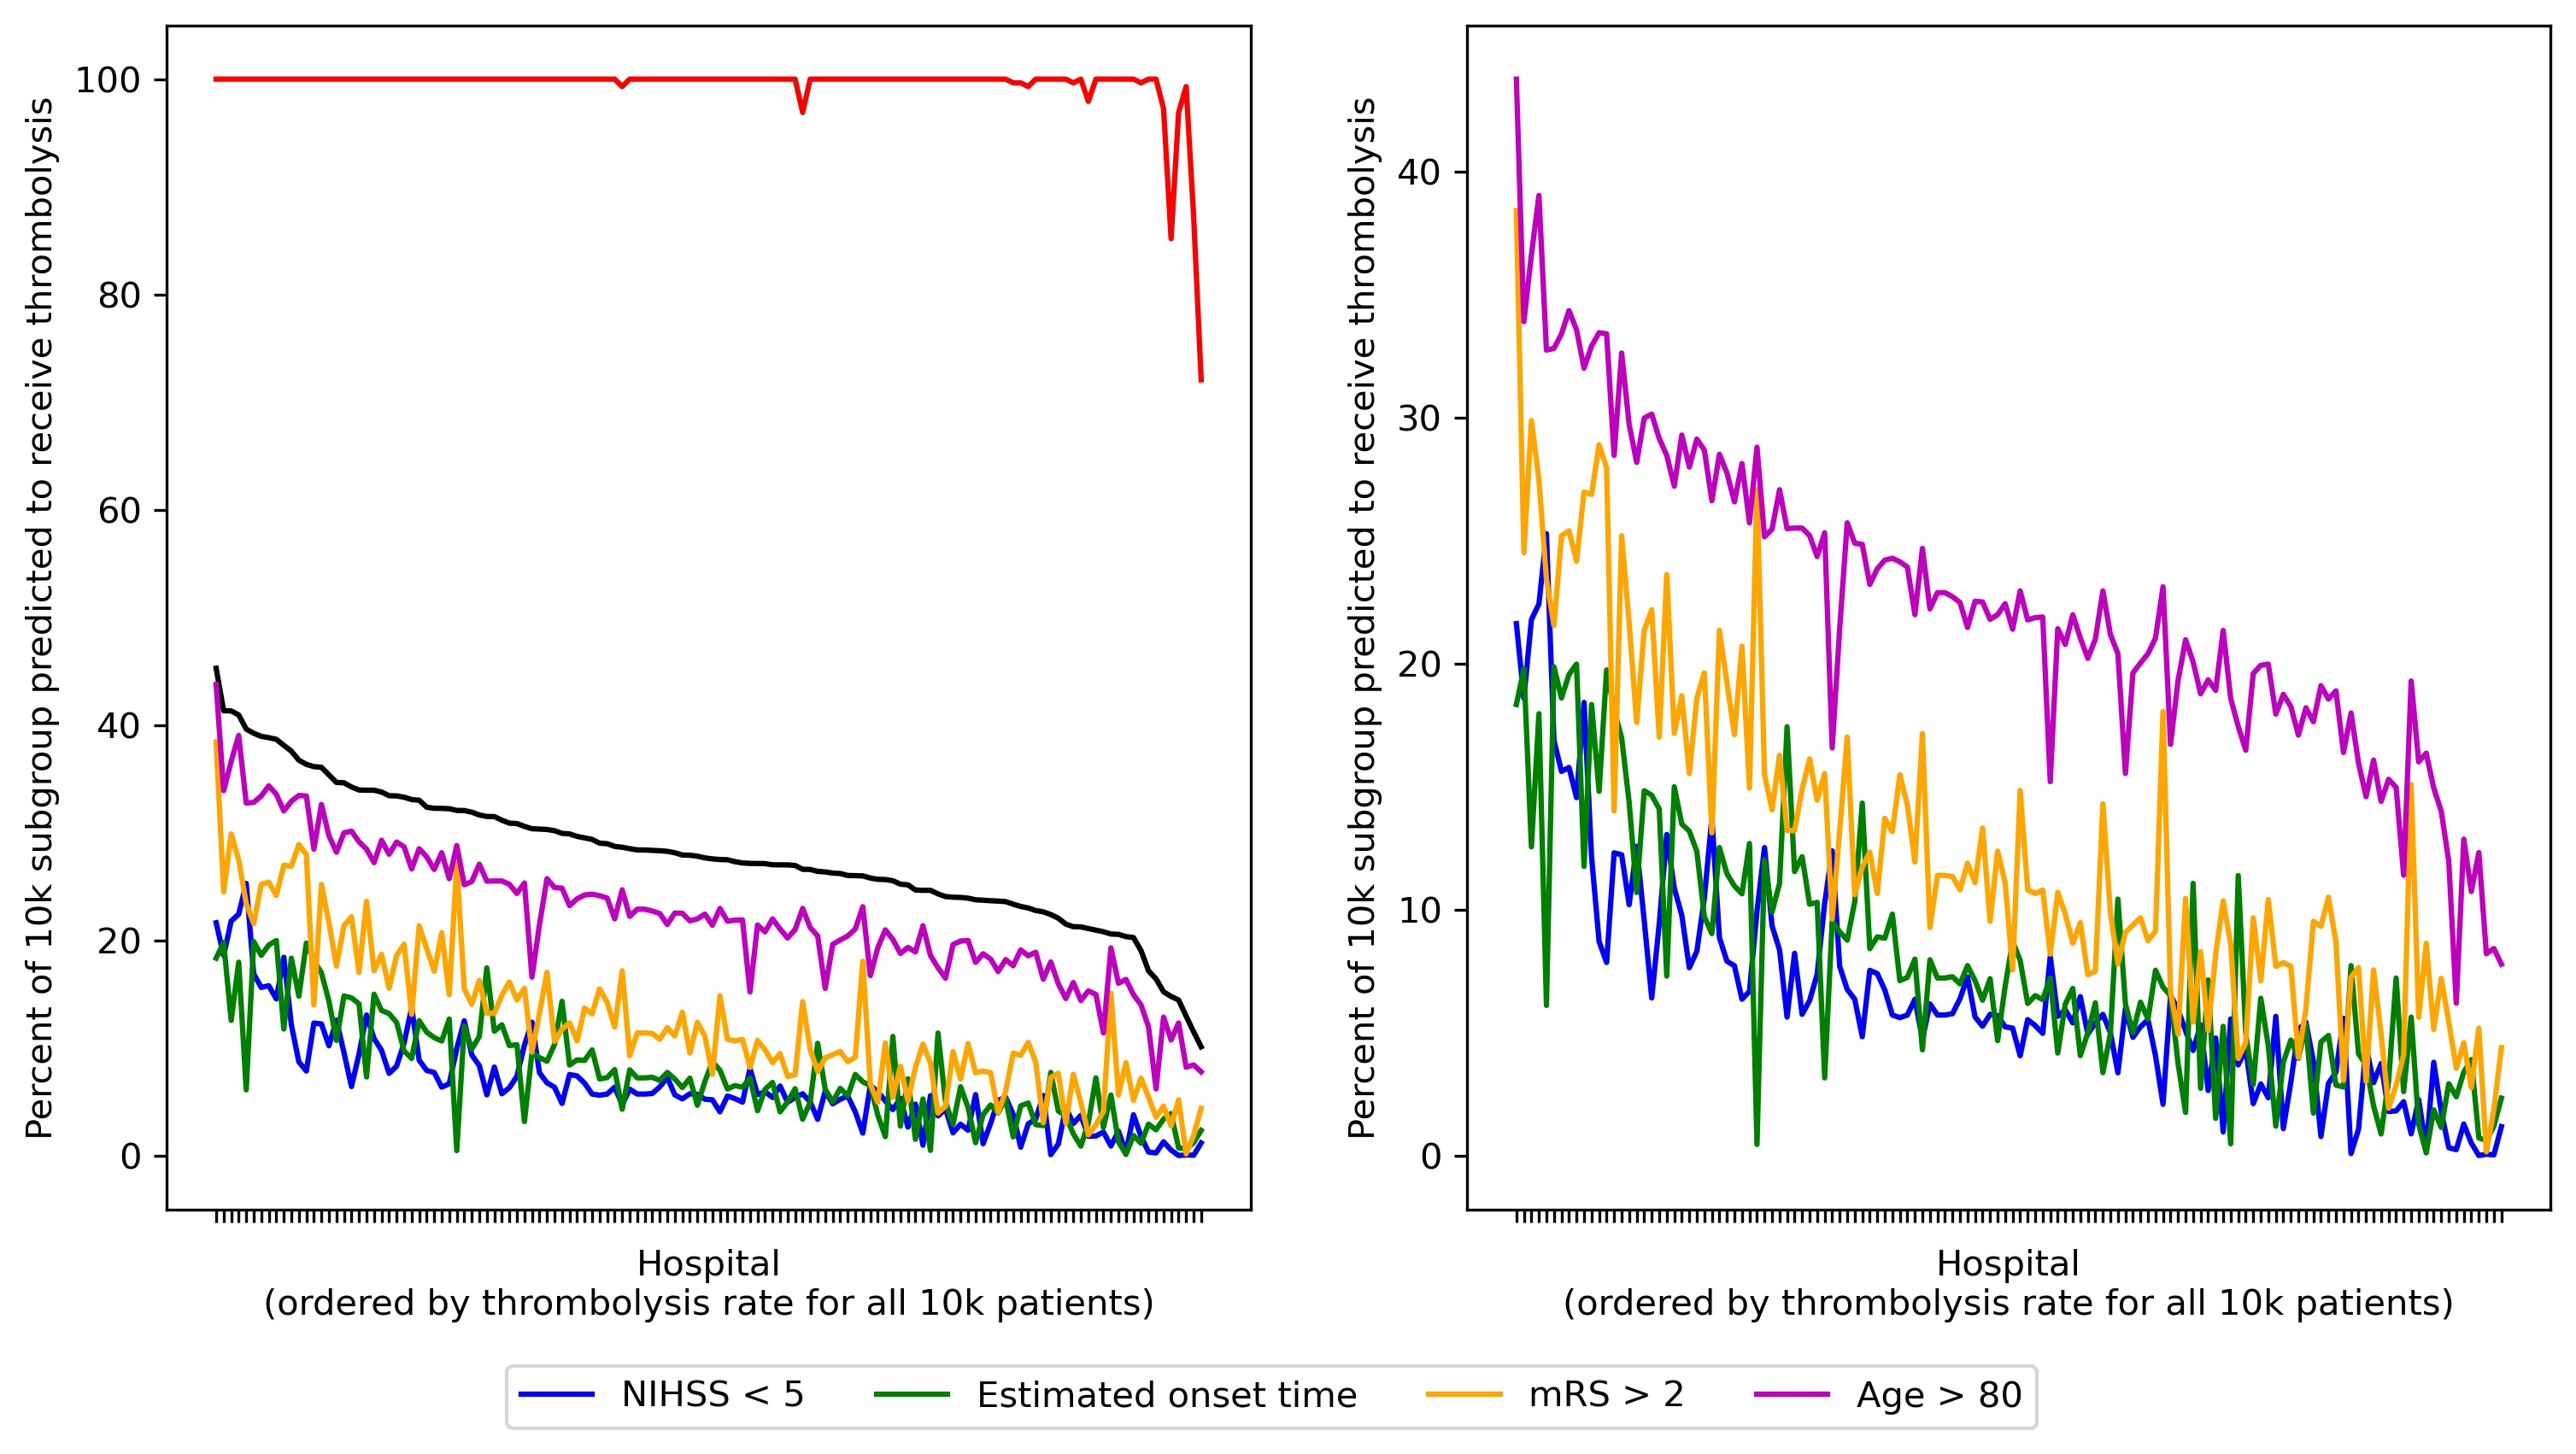
\includegraphics[width=0.95\textwidth]{./images/15_xgb_10_features_10k_cohort}
    \end{center}

\footnotesize Hospitals with lower thrombolysis use were particularly less likely to give thrombolysis to patients with milder strokes, prior disability, or patients with imprecise onset time.
\newline
\newline
\footnotesize Note: Subgroups, other than \emph{ideal patients}, tend to track each other.  

\end{frame}
\begin{frame}
\frametitle{We can predict what decision each hospital would make on different patients}

\vspace{3mm}

\begin{columns}[t]
    \begin{column}{0.45\textwidth}
        Base patient:
        \begin{itemize}
            \footnotesize
            \item Onset to arrival = 80 mins
            \item Arrival to scan = 20 mins
            \item Infarction = Yes
            \item NIHSS = 15
            \item Prior disability level = 0
            \item Precise onset time = Yes
            \item Use of AF anticoagulents = No
        \end{itemize}
    \end{column}
    
    \begin{column}{0.5\textwidth}
    \color{teal}
    Proportion of hospitals predicted to give thrombolysis:
    \footnotesize
    \begin{itemize}
        \color{teal}
        \item Base patient: 99\%
    \end{itemize}
    %\pause{} %Creates 2 PDF slides with pause here
    \vspace{3mm}
    \normalfont
    \color{red}
    \normalsize
    Base patient with:
    \footnotesize
    \begin{itemize}
        \color{red}
        \item NIHSS = 4: 73\%
        \item Pre-stroke mRS = 3: 86\%
        \item Estimated stroke onset time: 64\%
    \end{itemize}
    \end{column}

\end{columns}

\vspace{7mm}
This allows us to open up discussions between hospitals on differences in choices around thrombolysis.
\end{frame}

\begin{frame}
\frametitle{Investigating how hospitals differ in thrombolysis decision-making: Artificial patients}

\begin{center}
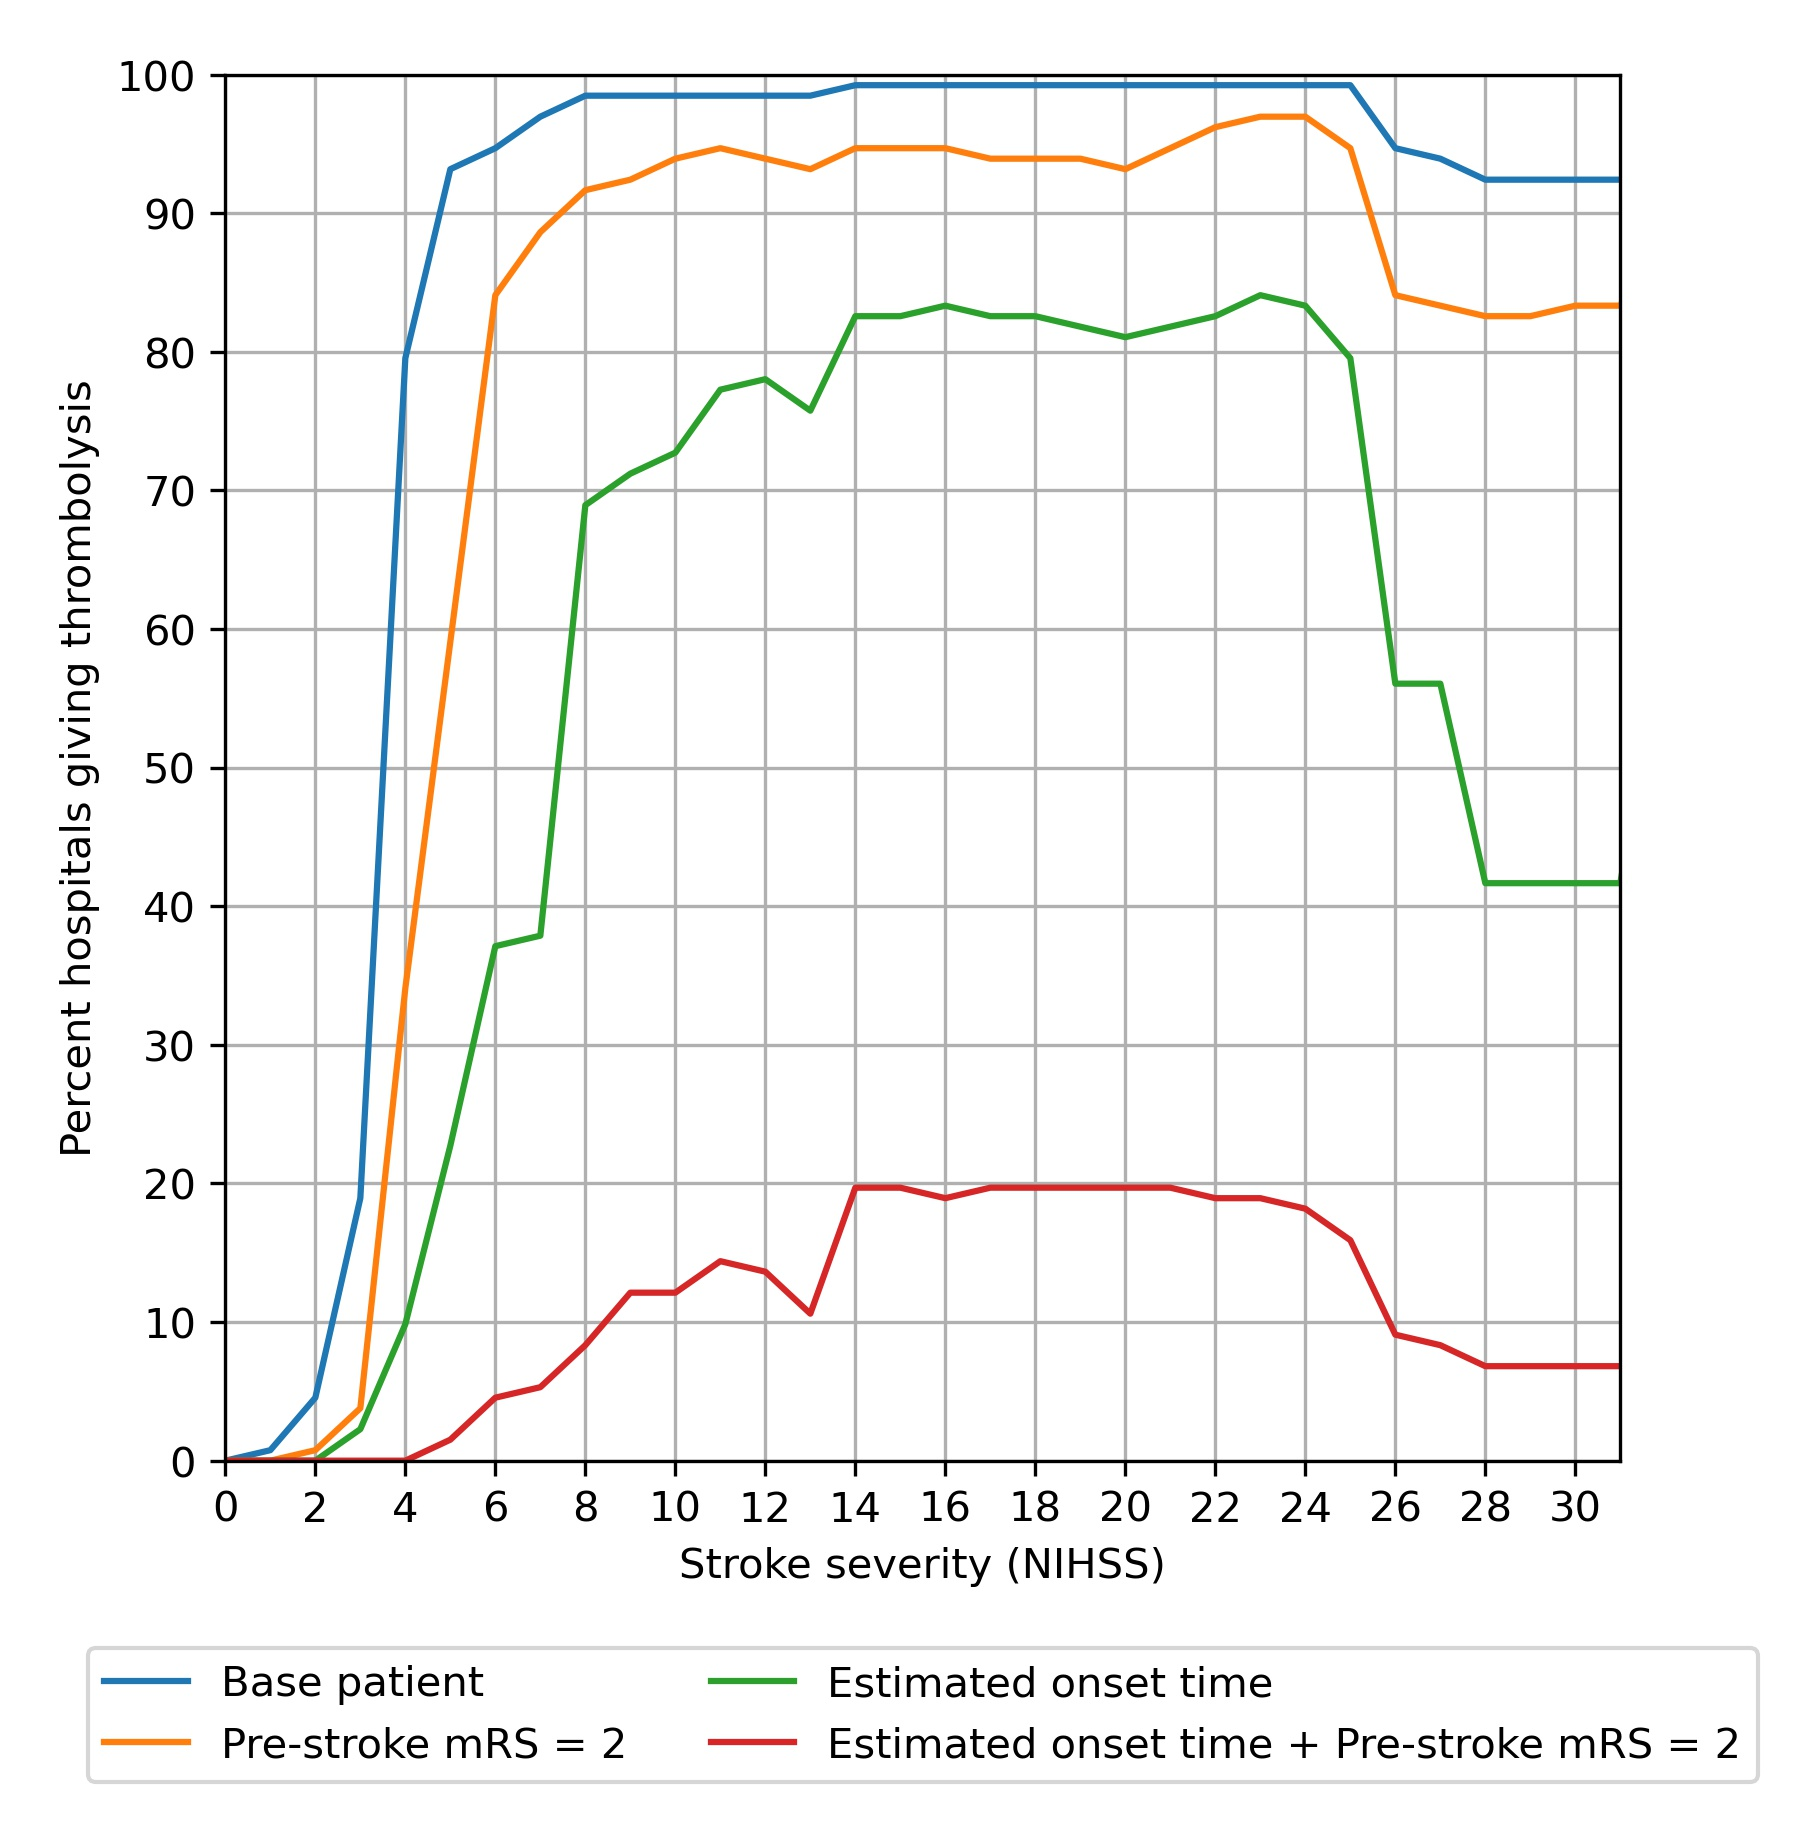
\includegraphics[width=0.7\textwidth]{./images/20_synthetic_xgb_10_features_interactions}
\end{center}


\end{frame}

\begin{frame}
\frametitle{How would different teams respond to the same patient?}

    \begin{center}
    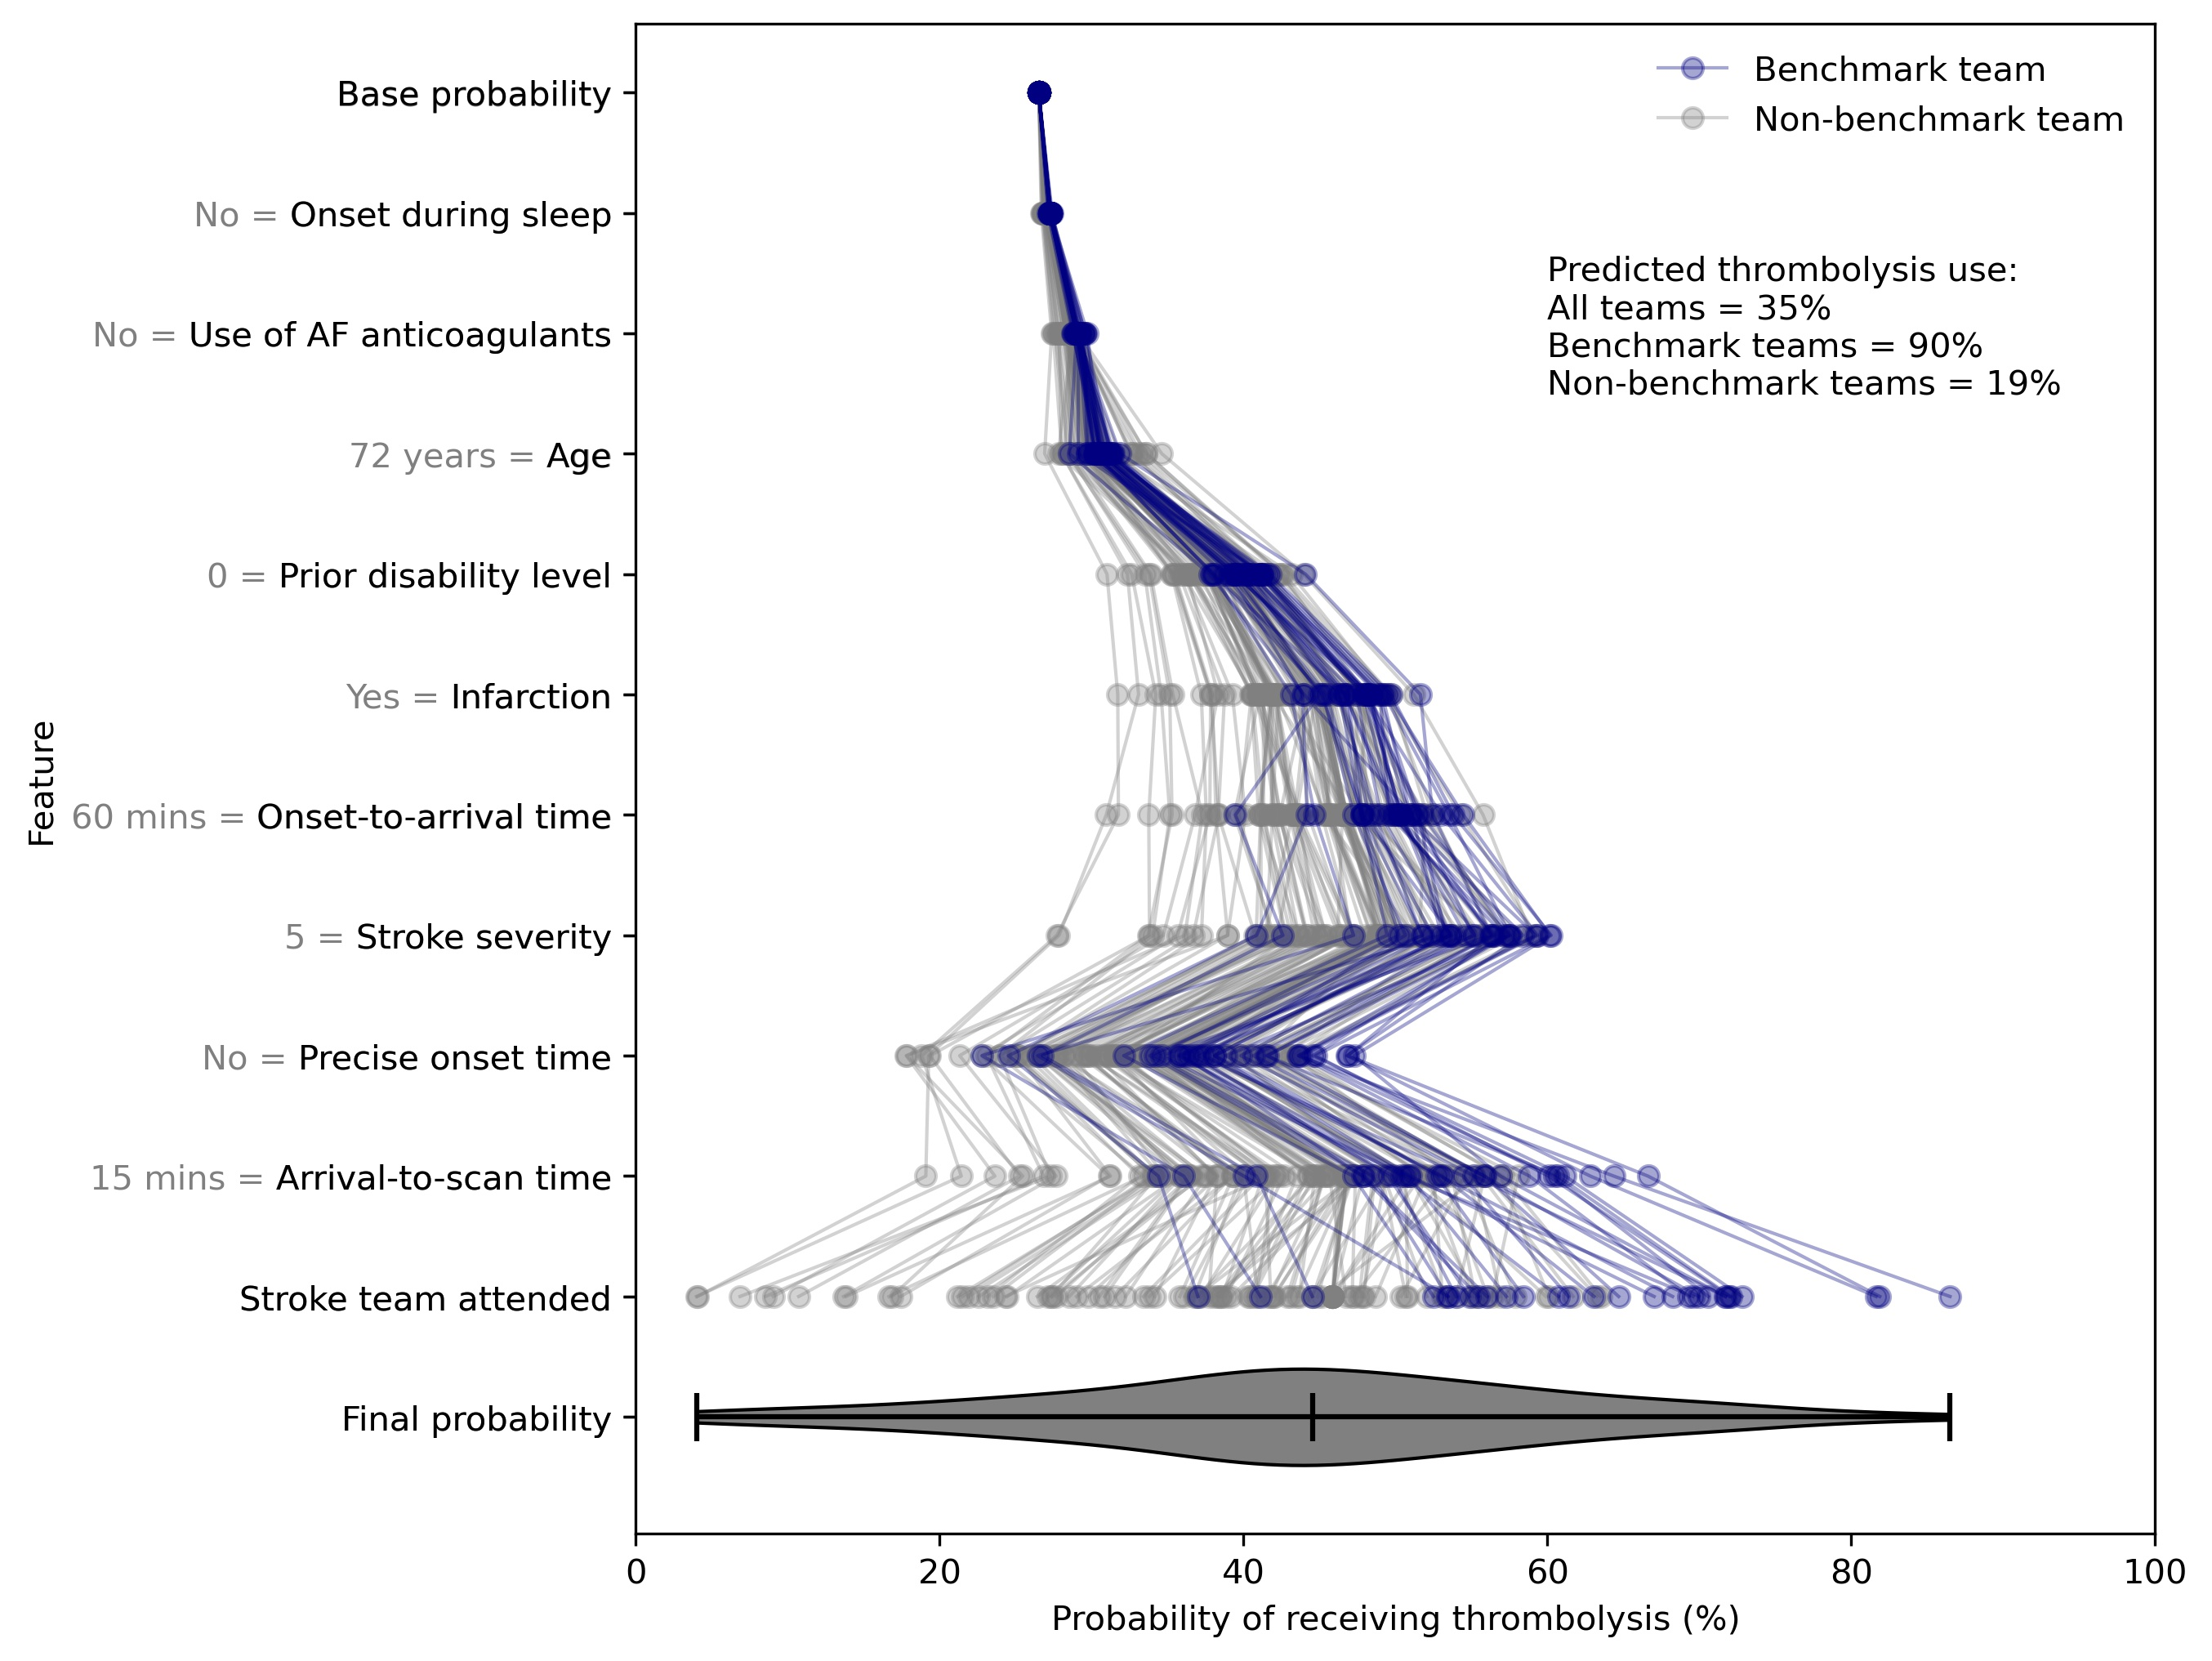
\includegraphics[width=0.7\textwidth]{./images/21_shap_waterfall_with_violin_contentious.jpg}
    \end{center}

\footnotesize The patient starts with the same base probability, then each hospital reacts differently when presented with each of the patients characteristics and nudges the probability to a different level.

\end{frame}


\begin{frame}
\frametitle{Summary}
\small

\begin{itemize}
    \item The XGBoost/SHAP model revealed that the odds of receiving thrombolysis:
    
    \begin{itemize}
        \scriptsize
        \item Reduced 20 fold over the first 100 minutes of arrival-to-scan time.
        \item Varied 30 fold depending on stroke severity.
        \item Reduced 3 fold with imprecise onset time.
        \item Fell 5 fold with increasing pre-stroke disability.
        \item Varied 15 fold between hospitals. 
        \item Fell 5 fold if the patient was taking anticoagulant medication.
        \item Was stable for the first two hours of arrival-to-onset time, and then fell 3 fold between two and four hours arrival-to-onset time
        \item Fell 2 fold between the age of 80 and 110.
        \item Fell 4 fold if onset was during sleep (these patients will also have the reduction due to imprecise onset time). 
    \end{itemize}

\small
\item The hospital identification (hospital SHAP value) explained 58\% of the variance in between-hospital thrombolysis use. 

\item Hospitals with lower thrombolysis use were particularly less likely to give thrombolysis to patients with milder strokes, prior disability, or patients with imprecise onset time.

\end{itemize}

\end{frame}


%%%%%%%%%%%%%%%%%%%%%%%%%%%%%%%%%%%%%%%%%%%%%%%%%%%%%%%%%%%%%%%


\end{document}




